%
% this file is encoded in utf-8
% v2.0 (Apr. 5, 2009)

\documentclass[12pt, a4paper]{ntuthesis}

% 除非校方修改了論文格式 (margins, header, footer, 浮水印, 中文數字之章別)
% 或者需要增加所用的 LaTeX 套件,
% 或者要改預設中文字型、編碼
% 否則毋須修改本檔內容
% 論文撰寫,請修改以 my_  開頭檔名的各檔案

\usepackage{CJKutf8}  %%% ZZZ %%% macro for Chinese/Japanese/Korean processing
\usepackage{CJKnumb} %%% ZZZ %%% for Chinese numbering capability
\usepackage[nospace]{cite}  % for smart citation
%\usepackage{geometry}  % for easy margin settings
\usepackage{ntuthesis}
\usepackage{multirow,multicol,rotating}

%
% margins setting
%\geometry{verbose,a4paper,tmargin=3.5cm,bmargin=2cm,lmargin=4cm,rmargin=2cm}
%

% 插圖套件 graphicx
% 使用者工作流程是用 pdftex 還是 latex + dvipdfmx?
% 視情況而有不同的參數
% 這裡作自動判斷
% 參考自
% http://www.tex.ac.uk/cgi-bin/texfaq2html?label=ifpdf
\newcommand\mydvipdfmxflow{dvipdfmx}
\newcommand\mypdftexflow{pdftex}
\ifx\pdfoutput\undefined
  % not running pdftex
  \usepackage[dvipdfm]{graphicx}
  \newcommand\myworkflow{dvipdfmx}  % set the flag for hyperref
\else
  \ifx\pdfoutput\relax
    % not running pdftex
    \usepackage[dvipdfm]{graphicx}
    \newcommand\myworkflow{dvipdfmx}  % set the flag
  \else
    % running pdftex, with...
    \ifnum\pdfoutput>0
      % ... PDF output
      %\usepackage[pdftex]{graphicx}
      \newcommand\myworkflow{pdftex}  % set the flag
    \else
      %...DVI output
      \usepackage[dvipdfm]{graphicx}
      \newcommand\myworkflow{dvipdfmx}  % set the flag
    \fi
  \fi
\fi

% 增強功能型頁楣 / 頁腳套件
\usepackage{fancyhdr}  % 借用此套件來擺放浮水印 
% (佔用了 central header)
% 不需要浮水印的使用者仍可利用此套件,產生所需的 header, footer
%
% 啟動 fancy header/footer 套件
\pagestyle{fancy}
\fancyhead{}  % reset left, central, right header to empty
\fancyfoot[C]{\thepage} %中間 footer 擺放頁碼
\renewcommand{\headrulewidth}{0pt} % header 的直線; 0pt 則無線

% 如果不需要任何浮水印,則請把下列介於 >>> 與 <<< 之間
% 的文字行關掉 (行首加上百分號)
%% 浮水印 >>> 
%\input{yzu_watermark.tex}
%% <<< 浮水印

% 如需額外的頁楣 (header) 或 footer,請在 my_headerfooter.tex 裡依例修改
% 它的預設內容是都關掉,可依需要打開
\input{my_headerfooter.tex}



%%%%%%%%%%%%%%%%%%%%%%%%%%%%%%
%%%% 非必要的套件,但很實用
\usepackage{amsmath} % 各式 AMS 數學功能
\usepackage{amssymb} % 各式 AMS 數學符號
\usepackage{mathrsfs} %草寫體數學符號,在數學模式裡用 \mathscr{E} 得草寫 E
\usepackage{listings} % 程式列表套件
\usepackage{subfig}
\usepackage{tabularx,colortbl}
\usepackage{url}
\usepackage[usenames,dvipsnames]{xcolor}
\usepackage{pgf}
\usepackage{tikz}
\usetikzlibrary{arrows,automata,positioning}



% Title Page
\renewcommand{\enTitle}{Multilingual Acoustic Modeling in Automatic Speech Recognition Using Deep Learning}  %英文標題
\renewcommand{\zhTitle}{深度學習多語言下的語音辨識聲學模型}  %中文標題
\renewcommand{\authorZhName}{呂相弘}  %作者中文姓名
\renewcommand{\authorEnName}{Hsiang-Hung, Lu}  %作者英文姓名
\renewcommand{\authorStudentID}{R03942039}  %作者學號
\renewcommand{\advisorZhName}{李琳山}  %指導教授中文姓名
\renewcommand{\advisorEnName}{Lin-Shan Lee}  %指導教授英文姓名
\renewcommand{\zhCollegeName}{電機資訊學院}  %學院中文名稱
\renewcommand{\enCollegeName}{College of Electrical Enginnering and Computer Science}  %學院英文名稱
\renewcommand{\zhDepartmentName}{電信工程學研究所}  %系所中文名稱
\renewcommand{\enDepartmentName}{Graduate Institute of Communication Engineering}  %系所英文名稱
\renewcommand{\rocYear}{一百零五}  %中華民國紀年年份
\renewcommand{\zhMonth}{七}  %中文月份
\renewcommand{\enYear}{2016}  %公元紀年
\renewcommand{\enMonth}{July}  %英文月份
\renewcommand{\oralDate}{105 年 7 月 xx 日}  %口試日期

%
% listing setting
\lstset{breaklines=true,% 過長的程式行可斷行
extendedchars=false,% 中文處理不需要 extendedchars
texcl=true,% 中文註解需要有 TeX 處理過的 comment line, 所以設成 true
comment=[l]\%\%,% 以雙「百分號」做為程式中文註解的起頭標記,配合 MATLAB
basicstyle=\small,% 小號字體, 約 10 pt 大小
commentstyle=\upshape,% 預設是斜體字,會影響註解裏的英文,改用正體
%language=Octave % 會將一些 octave 指令以粗體顯示
}

\usepackage{url} % 在文稿中引用網址,可以用 \url{http://www.yzu.edu.tw} 方式

%%%% 以上為非必要套件
%%%%%%%%%%%%%%%%%%%%%%%%%%%%%%

%%% 以下是 hyperref 套件
%%%%%%%%%%%%%%%%%%%%%%%%%%%%%%
% hyperref 會擾亂 cite.sty 對文獻號碼縮編的排版,所以依據
% http://www.ctan.org/tex-archive/macros/latex/contrib/hyperref/
% 作如下的更動,使得 hyperref 不做文獻號碼的超連結。
\makeatletter
\def\NAT@parse{\typeout{This is a fake Natbib command to fool Hyperref.}}
\makeatother

% hyperlinkable table of contents
% 章節目錄、圖表超連結
\ifx\myworkflow\mydvipdfmxflow
	\usepackage[dvipdfmx, debug, colorlinks, linkcolor=black, citecolor=black, urlcolor=black, unicode]{hyperref}
\else
	\usepackage[pdftex, debug, colorlinks, linkcolor=black, citecolor=black, urlcolor=black, unicode]{hyperref}	
\fi

% if hyperref is not used (e.g., in LyX application)
% define dummy \phantomsection for those occurences
%   in yzu_frontpages.tex, yzu_backpages.tex, my_appendix.tex
\ifx\hypersetup\undefined
	\newcommand\phantomsection{}
\fi

% hyperref跟algorithm衝突,hyperref必須放在algorithm前面
\usepackage{algorithm}
\usepackage{algorithmic}
%%%% 以上為所有套件
%%%% 
%%%% 

% global page layout
%\newcommand{\mybaselinestretch}{1.5}  %行距 1.5 倍 + 20%, (約為 double space)
%\renewcommand{\baselinestretch}{\mybaselinestretch}  % 論文行距預設值
%\parskip=2ex  % 段落之間的間隔為兩個 x 的高度
%\parindent = 0Pt  % 段首內縮由 CJK 控制,所以這裡就設成不內縮

%%%%%%%%%%%%%%%%%%%%%%%%%%%%%
%  end of preamble
%%%%%%%%%%%%%%%%%%%%%%%%%%%%%
%
\begin{document}
\begin{CJK}{UTF8}{bsmi}   %%% ZZZ %%%  <<< 在這裡更改預設中文字型、編碼
% 編碼:UTF8, Bg5, ...
% 中文字型名稱:TeXLive 安裝有一套明體字 bsmi, 楷書與其他字型視你的 LaTeX CJK 系統裝設情況而定

% 針對 latex + dvipdfmx 工作流程在 hyperref 套件的影響下,圖檔的辨識力退化
% 所作的權宜措施。可能是因為 TeXLive2007 hyperref 裏的
% 客製 graphicx / dvipdfmx 的設定檔不夠新
\ifx\myworkflow\mydvipdfmxflow
	\DeclareGraphicsExtensions{.pdf,.png,.jpg,.eps}
	\DeclareGraphicsRule{.pdf}{eps}{.bb}{}
	\DeclareGraphicsRule{.png}{eps}{.bb}{}
	\DeclareGraphicsRule{.jpg}{eps}{.bb}{}
\fi

% global CJK setting
\CJKindent  %%% ZZZ %%%  段首內縮兩格

% 載入中文名詞的定義:例如,Figure -->「圖」, Chapter -->「第 x 章」
\input{ntu_definitions.tex}

% 如果不需要以中文數字一、二、三呈現章別,例如「第一章」
% 則請把下列介於 >>> 與 <<< 之間
% 的文字行關掉 (行首加上百分號), 會以「第 1 章」呈現
%% 中文數字章別 >>>
\input{ntu_chnum.tex}
%% <<< 中文數字章別

%%% 以下是載入前頁、本文、後頁
% 請勿更動
% 如需針對個別章節獨立編譯
% 請在 my_chapters.tex 檔裡對個別章節的 \input 指令以行首百分號方式做開關。

\NTUtitlepage  % 產生論文封面

\newpage
\setcounter{page}{1}
\pagenumbering{roman}
%
%\NTUoralpage  % 產生口試委員會審定書

\mydoublespacing
\begin{acknowledgement} %誌謝
TODO誌謝
\end{acknowledgement}

\begin{zhAbstract}  %中文摘要
TODO摘要

\end{zhAbstract}

{
%\zhKaiFont
\mysinglespacing\selectfont
\tableofcontents %目錄

\listoffigures  %圖目錄

\listoftables  %表目錄
\par
}

\newpage
\setcounter{page}{1}
\pagenumbering{arabic}


\chapter{導論}
  \section{研究動機與背景}

長久以來,科技的發展早已走向花花綠綠,聲色斑駁的世代。絢爛的圖片影像、繁複錯落的聲音樂曲,連結人們日常生活的已經不再是書本上的文字,而是各種多媒體層層交疊的網路生活。其中,語音辨識應運而生,人們一邊訝異機器能夠把人的聲音訊號打成文字,一邊又享受機器聽懂人話後的各種方便福利。從最基本的的行動裝置語音輸入,後來的語音檢索,甚至發展成語音助理如Google Now, Microsoft Cortana及Apple Siri,都深深刻刻地使用了語音辨識及相關的語音處理技術。

隨著網路與相關科技的成長,語音辨識彷彿逆著馬斯洛的人類需求金字塔一般。一開始,人們追求語音辨識只不過是一種自我實現,展現科技的威能:而現在,語音辨識已經貼近人們的需求,居家照顧、生活機能等等廣泛的應用,使得人類越來越無法脫離這個方便迅速的「口說」世代。而這樣的發展顯然是全球化的,地球上無論是說著德文、西班牙文、英文還是中文的人,都無法抵抗這迅速發展的洪流,只能擁抱日益新穎的科技,融入日常。

語言的高度變化,一直以來都是語音辨識系統最大的挑戰。不同語系、不同腔調、非母語者甚至是不同使用者講的同一個語言,都不見得適用同一個系統。直觀而言,我們可以為每一個語言,建立一個獨自的語音辨識系統,然世界上語言何其多,語言之間也不必然完全獨立,各自為政不免冗贅。如何運用語言之間的共通特性,重複利用,進而適應各種可能的語音環境,是語音辨識中的核心課題。
\section{相關研究}
以往的語音辨識,都習慣將聲音拆解成不同層級的發單位,如語言學上的音素(Phoneme)、或是模擬發音連續狀態的三連音態(Tri-state, or senone)。當聲學模型(Acoustic Model)建立後,即與語言模型(Language Model)結合成辨識系統。
 
自從辛氏(Hinto)將深層類神經網路(Deep Neural Network, DNN)套用到聲學模型後,語音辨識系統的辨識率突飛猛進,研究者紛紛踏入深度學習的領域,試圖找尋更潛在的隱藏層(Hidden Layer)資訊。更有研究者直接跳脫語言學的知識,回歸問題的本質,建立了端至端(End-to-End)語音辨識系統,不再有音素或是發音狀態的概念,移除了語言學對於深度學習的框架限制。隨著網路頻寬的擴增的與大資料背景的加持,以往仰賴資料量的深度學習不再成為瓶頸,這些方法紛紛獲得顯著的成功。

深度學習的架構非常多元,大多是以類神經網路為基礎延伸而成。有能夠抓取圖像中空間頻率的卷積類神經網路(Convolutional Neural Network, CNN)、能夠抓取短期時間資訊的遞迴式類神經網路(Recurrent Neural Network, RNN)、利用閘道存取長時間時間資訊的長短期記憶神經網路(Long Short-term Memory, LSTM)等等。

儘管有這麼豐富的方法,多語言語音辨識系統中仍然有許多難以克服的情景。如原生語音辨識系統與非母語(Nonnative)或是不同地區腔調(Accented)使用者的不匹配問題(Mismatch)、雙語混和(Code-mixing)使用者的語言切換問題(Code-switching)。少數語言的資源過少問題(Low-resource)。這些問題,追根究底都是因為實際雲端資料庫中儲存的資料量不足,使得系統無法完善。常見的解決方法如發音單位合併(Pronunication Unit Merging)、多目標學習(Multitask Learning)、聲學模型共享(Acoustic Model Sharing)、跨語言轉移學習(Crosslingual Transfer Learning)、半監督式學習(Semi-supervised Learning),也都是從資料量的角度切入,擴增可用的資料,讓深度學習的結果變得更可靠。

為了避免深度學習過度適應(Overfitting)於少量的訓練資料,機器學習的研究者發展出控制調適(Regularization),像是隨機調適的丟棄演算法(Dropout)、模型簡單化的二階參數衰減法(L2 Weight Decay)、或是知識蒸餾演算法(Knowledge Distillation)。藉由控制調適,能夠提高深度學習模型的概括化能力(Generaliaztion),從而學習到少數資料量以外的更多可能。強力的控制子(Regularizer)甚至可以簡化模型的架構,讓小型的行動裝置亦能配備,增加應用可以運用的空間範圍。

\section{研究方向}
本論文之研究方向在探討以深度學習建立的多語言語音辨識系統聲學模型,主要包含以下幾點:

\begin{itemize}
\itemsep -2pt %reduce space between items
  \item  第一階段先探討多個語言間如何合作分享資訊,以用較少的資料獲得更好的辨識結果。

  \item  第二階段則探討如何利用知識蒸餾幫助多語言的深層類神經網路學習,提昇模型的概括化能力。

\end{itemize}
\section{章節安排}
本論文各章節簡述如下:
\begin{itemize}
\itemsep -2pt %reduce space between items
  \item  第二章:介紹深度學習的深層類神經網路架構與基本訓練方法,以及本論文研究所使用的語料全球音素資料庫(GlobalPhone Corpus)還有常見的多語言語音辨識系統情景。

  \item  第三章:建立四個語言:德文(German, GE)、西班牙文(Spanish, SP)、捷克文(Czech, CZ)、法文(French, FR)的單語言(Monolingual)語音辨識系統,以便之後的比較。為了讓深度學習的結果更適合討論與擴展而不受限於語言知識,因此筆者特別挑了四個完全不熟悉的語言。

  \item  第四章:建立四個語言的多語言(Multilingual)語音辨識系統,從最粗糙的音素到最細緻的隱藏層,合併三個不同層級的發音單位,並討論不同層級合併的意義與結果。

  \item  第五章:介紹如何以知識蒸餾來控制調適深度學習模型,並且設計實驗套用於多語言語音辨識系統上,進而討論模型壓縮與概括化的能力。
   
  \item  第六章:總結本論文的研究成果與研究精神,並討論未來的研究方向。
\end{itemize}


\chapter{背景知識}
  \section{深層類神經網路(Deep Neural Network, DNN)}    
\subsection{簡介}
深層類神經網路發想於生物的神經系統結構。神經系統由一層一層的神經元組成,彼此以樹突、軸突與突觸連結,每顆神經元自己有活化閾值來決定激發態與否。根據此仿生的觀察,便產生一種數學模型(如圖\ref{fig:chap2_neuron_a}與\ref{fig:chap2_neuron_b}),將神經元規劃為層狀結構(如圖\ref{fig:chap2_layer}),把輸入特徵(Input Features)通過一層一層的感知器(Perceptron)或稱隱藏層(Hidden Layer),傳遞到最後一層輸出層(Ouptut Layer),進行多類別分類(Multiclass Classification)或是回歸(Multiclass Regression)的監督式機器學習問題(Supervised Machine Learning Probelm)。因應圖形處理器(Graphics Processing Unit, GPU)的高度發展,適合平行多核運算的深層類神經網路獲得廣大社群的推薦與發展,儼然成為人人可以上手修改的技術,廣泛使用在不同的領域。

\begin{figure}
\centering
\subfloat[][生物學上的單顆神經元結構]{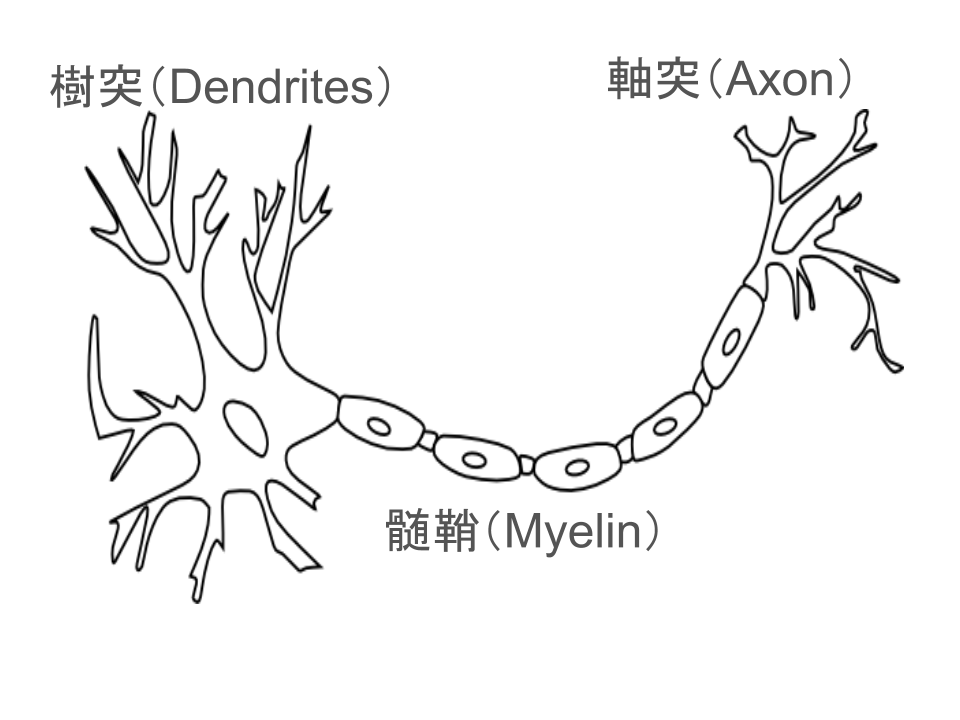
\includegraphics[scale=0.15]{images/chap2_neuron_a.png}\label{fig:chap2_neuron_a}}
\subfloat[][數學上的單顆神經元結構]{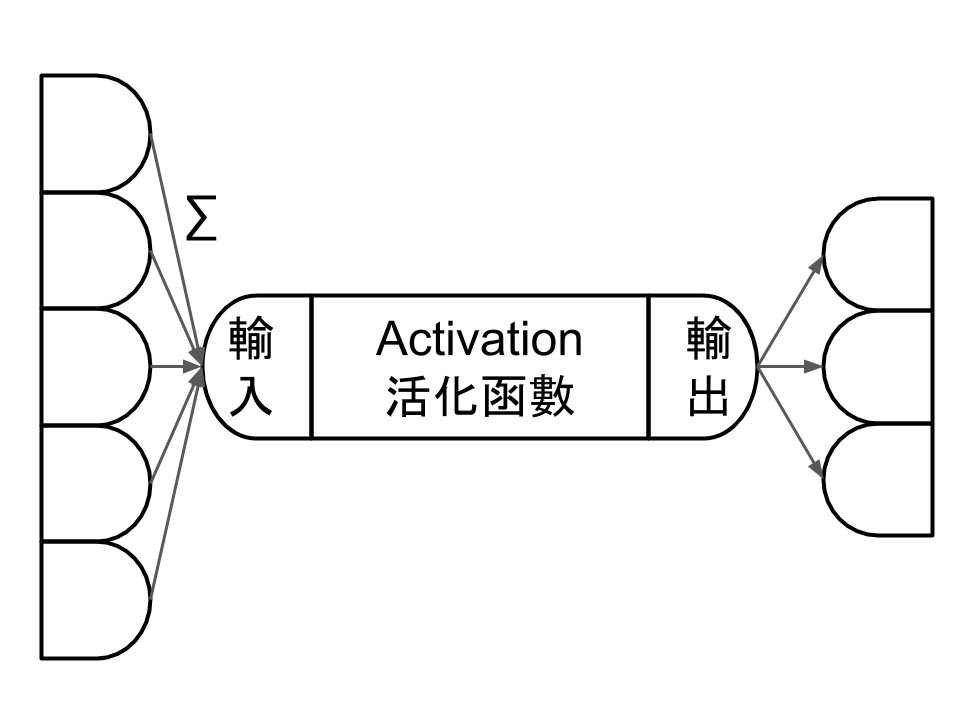
\includegraphics[scale=0.15]{images/chap2_neuron_b.png}\label{fig:chap2_neuron_b}}
\subfloat[][層狀連接的神經網路]{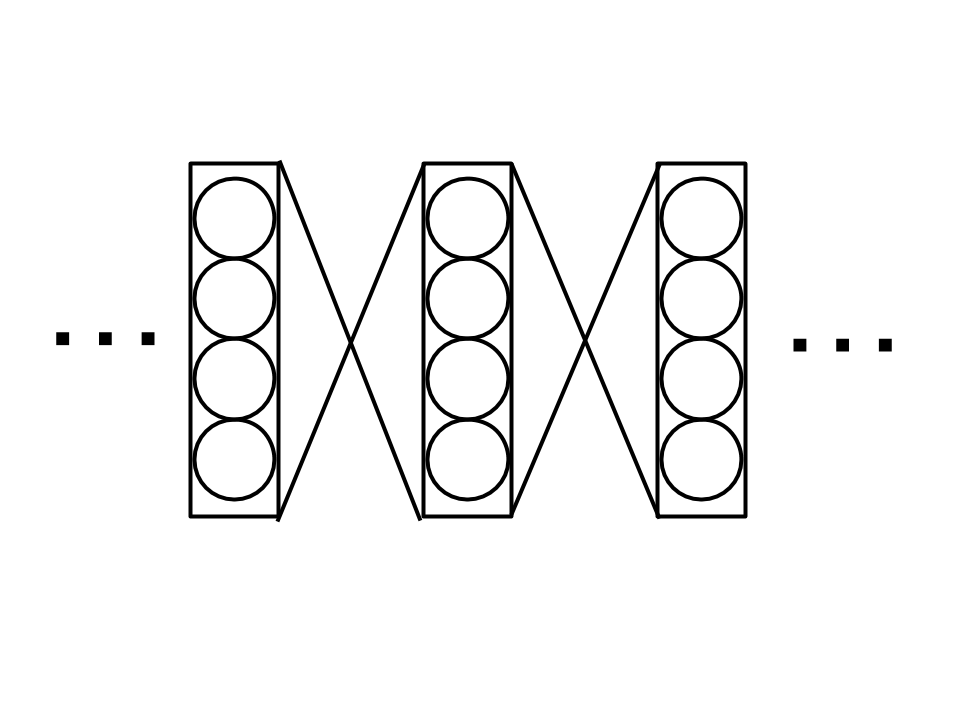
\includegraphics[scale=0.15]{images/chap2_layer.png}\label{fig:chap2_layer}}
\caption{類神經網路的基本架構}
\end{figure}

給定輸入特徵向量$\bold{x} = [x_1 , x_2 , x_3 , x_4 ... , x_D]^T$,與相應的標籤(Label)$\bold{y} = [y_1 , y_2 , y_3 , y_4 ... ,y_C]^T$,我們目標在取得最接近標籤的輸出$\bold{\hat{y}} = [\hat{y}_1 , \hat{y}_2 , \hat{y}_3 ... , \hat{y}_C]^T$。中間隱藏層$\bold{h^{(j)}} = [h^{(j)}_1 , h^{(j)}_2 , h^{(j)}_3 , h^{(j)}_4 ... , h^{(j)}_S]^T$的每一個神經元$h^{(j)}_{i}$都會經由仿射變換(Affine Transform)與非線性活化函數(Nonlinear Activation Function)後輸出。

仿射變換乃計算前一層所有神經元的輸出,進行加權總和(Weighted Summation)和閾值偏移(Threshold bias)。整體的數學式可表示成:
\begin{equation}
h^{(j)}_{i} =
\left\{\begin{matrix}
 \sigma (\sum_{k=1}^{S} w_{ki}^{j}h_{k}^{(j-1)} + b_{i}^{(j)}) & j = 2 , 3 , 4 ... H \\ 
 \sigma (\sum_{k=1}^{D} w_{ki}^{j}x_{k} + b_{i}^{(j)}) & j = 1 
\end{matrix}\right.
\end{equation}

其中$h_i^{(j)}$為第j層隱藏層的第i個神經元輸出;$\sigma$為活化函數;$w_{ki}^{(j)}$與 $b_{i}^{(j)}$分別為神經元突觸權重與活化閾值偏移;S為每一層隱藏層的寬度,代表每層包含的神經元數量;D為輸入層的維度;H為隱藏層的層數。這些都是設計模型的核心參數。

常見的活化函數有兩種,如S型函數(Sigmoid)和整流線性單元(Rectified Linear Unit, ReLU),分別為:
\begin{equation}
sigmoid(x) = \frac{1}{1 + e^{-x}}
\end{equation}
\begin{equation}
ReLU(x) = max( 0 , x )
\end{equation}
深層類神經網路的最後一層亦是仿射變換,但是不再經過活化函數,該層輸出又稱邏輯子(Logits):
\begin{equation}
z_i = \sum_{k=1}^{D} w_{ki}^{(H)}h_{k}^{(H)} + b_{i}^{(H)} 
\end{equation}
當深層類神經網路用作多類別的分類器時,邏輯子會通過軟性最大化轉換(Softmax),變成類似機率分佈的分類輸出:
\begin{equation} \label{eq:softmax}
\hat{y}_i = \frac{e^{z_i}}{\sum_{k=1}^{C}e^{z_k} }
\end{equation}
當深層類神經網路用作多類別的回歸器時,則直接輸出邏輯子的值:
\begin{equation}
\hat{y}_i = z_i 
\end{equation}
深層類神經網路便是藉由每一層權重矩陣$\bold{W}^{(h)} = \{w_{ij}^{(h)}\}$與每一層的偏移閾值$\bold{b}^{(h)}$,將一筆輸入資料$\bold{x}$轉換成輸出資料$\hat{\bold{y}}$的非線性函數$f_{\theta}:\mathbb{R}^D\rightarrow \mathbb{R}^C$,其中$\theta$為DNN的模型參數,也就是上述的權重矩陣與偏移閾值。使用DNN的核心問題,在於如何找到理想的函數$f_{\theta}$,已達到更高的分類準確率或是更少的回歸誤差。
\subsection{訓練方法}
DNN的訓練方式,需要借助損失函數(Loss Function),來模擬DNN與理想函數的量化距離。其訓練的目標可以規化為以下的最佳化問題(Optimization Problem):
\begin{equation}
\min_{\theta}{ \sum_{n=1}^{N}{ {L( \bold{x}_n , \bold{y}_n , \theta)}}}
\end{equation}
其中,$\bold{x}_n$為訓練輸入實例,總共有$N$個。$L(\bold{x}_n , \bold{y}_n, \theta)$為輸入實例$\bold{x}_n$通過模型$\theta$與正確標籤$\bold{y}_n$相比產生的損失。

一般來說,損失函數是模型設計者將真正的期望目標,與類神經網路的輸出結果相比算出來的距離。損失函數的值越大,代表模型的輸出結果與期望目標相差越遠,也因此訓練的目標為最小化損失函數。

以多類別分類器而言,分類器的輸出向量$\hat{\bold{y}}$,會將每一個維度對應到一個分類標籤,總共有$C$種類別。給定的正確標籤$\bold{y}$會公式化為1-hot向量$[0 , 0 , ... , 0 , 1 , 0 ... , 0]^T $,只有正確類別$l$的值是1,其餘為0。訓練此種分類器時,損失函數為交叉熵(Cross Entropy, CE),定義為:
\begin{equation} \label{eq:LCE}
L_{CE}(\bold{x} , \bold{y} , \theta) = KL( \bold{y} || f_{\theta}(\bold{x}) ) = KL(\bold{y} || \hat{\bold{y} }) = \sum_{i = 1}^{C} y_i \log{ \frac{y_i}{\hat{y}_i} } = - \log \hat{y}_{l} 
\end{equation}

其中$KL(p||q)$代表的是克雷散度(Kullback–Leibler Divergence),用以衡量兩組機率分佈的距離,值越大則代表兩組分佈越不相似。$L_{CE}$計算了分類器的正確標籤$\bold{y}$與通過模型參數後的預測向量$\hat{\bold{y}}$的克雷散度,但由於$C$種正確標籤中,只有一個類別$l$的值為1,也因此$L_{CE}$可以簡化成公式\ref{eq:LCE}最右邊的簡單型態,最小化正確分類標籤的負對數可能性(Negative Log Likelihood, NLL)。

以多類別回歸器而言,則更廣義地希望將回歸器的輸出向量$\hat{\bold{y}}$與目標向量$\bold{y}$的距離拉近。訓練此種分類器時,距離的衡量通常為均方差(Mean Square Error, MSE),定義為:
\begin{equation}
L_{MSE}(\bold{x} , \bold{y} , \theta) = || \bold{y} - f_{\theta}(\bold{x}) ||_2 = || \bold{y} - \hat{\bold{y}} ||_2 = \sum_{i = 1}^{C} ( y_i - \hat{y}_i )^2 
\end{equation}

當模型設計者決定好適當的損失函數後,下一個問題便是選擇解決最佳化問題的演算法。理想上,理想參數應能夠最小化損失函數:
\begin{equation}
\theta^* = \arg\min_{\theta}{ \sum_{n=1}^{N}{ {L( \bold{x}_n , \bold{y}_n , \theta)}}}
\end{equation}

但是因為DNN中間飽含非線性活化函數的緣故,最小化損失函數通常沒有方便可得的解析解(Analytical Solution),或稱封閉解(Close-form Solution)。實務上,通常採用迭代式(Iterative)演算法,給定一個參數起點,一步一步減少損失函數。
最簡單的迭代式最佳化演算法為統計式梯度降低(Stochastic Gradient Descent)演算法,給定某一組參數$\theta$,損失函數沿著該參數上的梯度方向更新,下降的速度最快,可表達成:
\begin{equation}
\theta_{k+1} \leftarrow \theta_k - \eta \Delta \theta_{k} 
\end{equation}
\begin{equation}
\Delta \theta_{k} = \frac{\partial L}{\partial \theta} \biggr|_{\theta = \theta_k}
\end{equation}
其中$\eta$為學習比率(Learning rate),調控最佳化的速度與精細度,$k$為更新的階段,隨著$k$的增加,可期望損失函數的值越來越小,模型越接近理想模型。

然而梯度的計算牽扯到函數的一次微分,對於雜訊的反應較不穩健,訓練上不穩定。更進階的訓練方式包含了慣量(Momentum),使得每次SGD更新的時候,包含了前次更新的梯度方向,可表達為:
\begin{equation}
\Delta \theta_{k} =  \mu \Delta \theta_{k-1} + \frac{\partial L}{\partial \theta} \biggr|_{\theta = \theta_k}
\end{equation}
其中$\mu$為慣量係數,用以調控慣量的比例。

在使用SGD訓練DNN的時候,通常是使用反向傳播(Back Propagation)演算法,在DNN完成順向預測(Forward Prediction)計算出$\hat{\bold{y}}$後,會先得到最後一層參數的梯度值,再根據鏈鎖律(Chain-rule),將梯度反向傳播回輸入層,取得每一層的參數的梯度值,從而完成一次更新。
使用最佳化演算法訓練DNN的時候,沒有任何方法可以保證損失函數是下凹(Convex)的。在損失函數下降的過程中,並不保證會下降到最佳解(Global Optimum)上,很有可能會停在局部最佳解(Optimal, or Local Optimum)上。因此在訓練之初通常使用隨機初始化,並且擴增模型的隨機性,以避免掉落到結果較差的局部最佳解上。

\begin{figure}
\centering
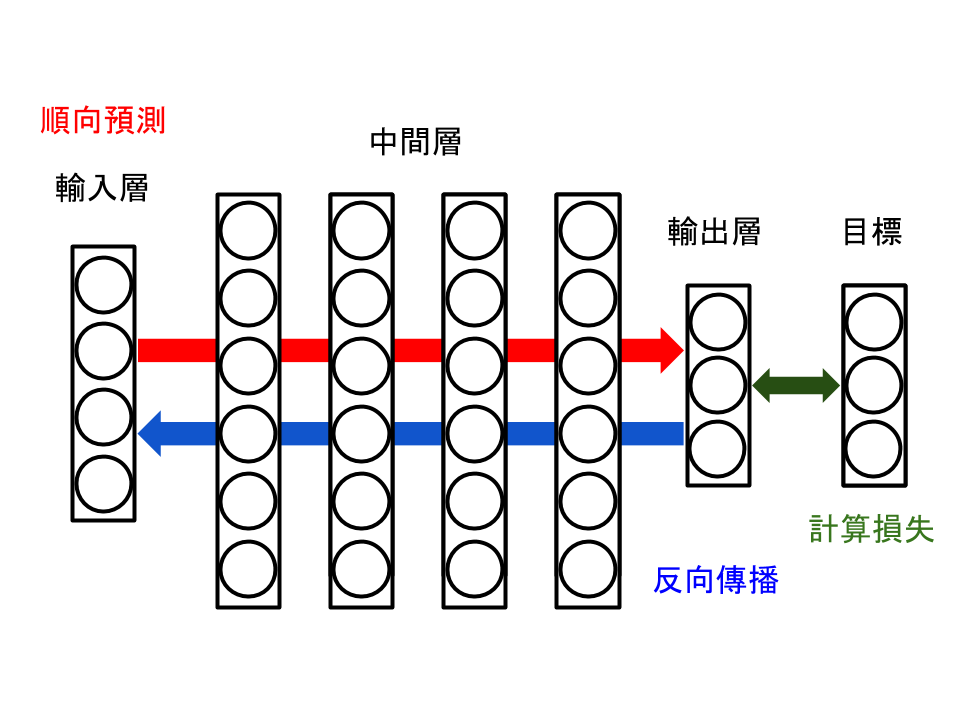
\includegraphics[scale=0.35]{images/chap2_dnn.png}
\caption{深層類神經網路訓練示意圖}
\label{fig:chap2_dnn}
\end{figure}

\subsection{丟棄演算法}
所有的機器學習模型,都會陷入過度適應(Overfitting)的情況。發生過度適應時,模型能夠在訓練集上達到很好的表現,卻在測試集上表現得越來越差。這時候模型的概括化的能力正逐漸下降,而是單純記憶輸入資料的規律與數字,無法學習到真正幫助辨識學習的本質。
最常見避免過度適應的方法,就是使用控制調適(Regularization)。使用控制調適,可以縮減模型複雜度,卻不會縮減模型強度,如在損失函數上額外添加控制參數大小的控制子。針對DNN,辛氏提出了丟棄演算法(Dropout):順向預測時,每個神經元會有$p$的機率直接關閉,無法活化,使得輸出值為$0$,如圖\ref{fig:chap2_dropout_b}與圖\ref{fig:chap2_dropout_c}。藉由隨機丟棄,可以強迫模型中的各種參數自力更生,而不是相互適應,強迫模型學到更概括化的能力。


\begin{figure}
\centering
\subfloat[][未經丟棄的DNN]{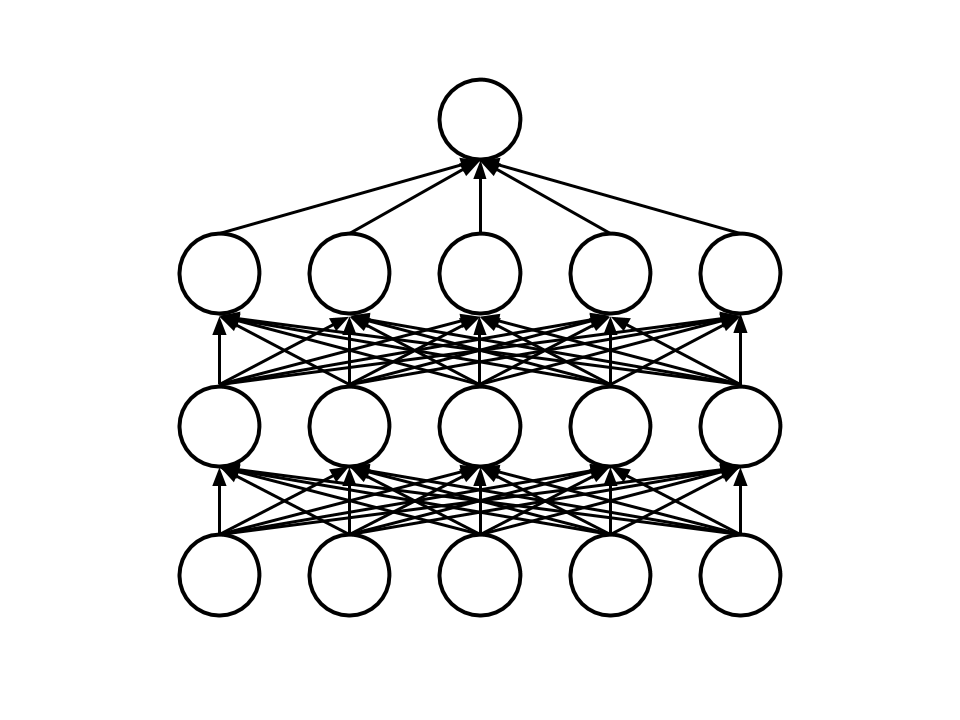
\includegraphics[scale=0.15]{images/chap2_dropout_a.png}\label{fig:chap2_dropout_a}}
\subfloat[][隨機丟棄部份神經元的DNN]{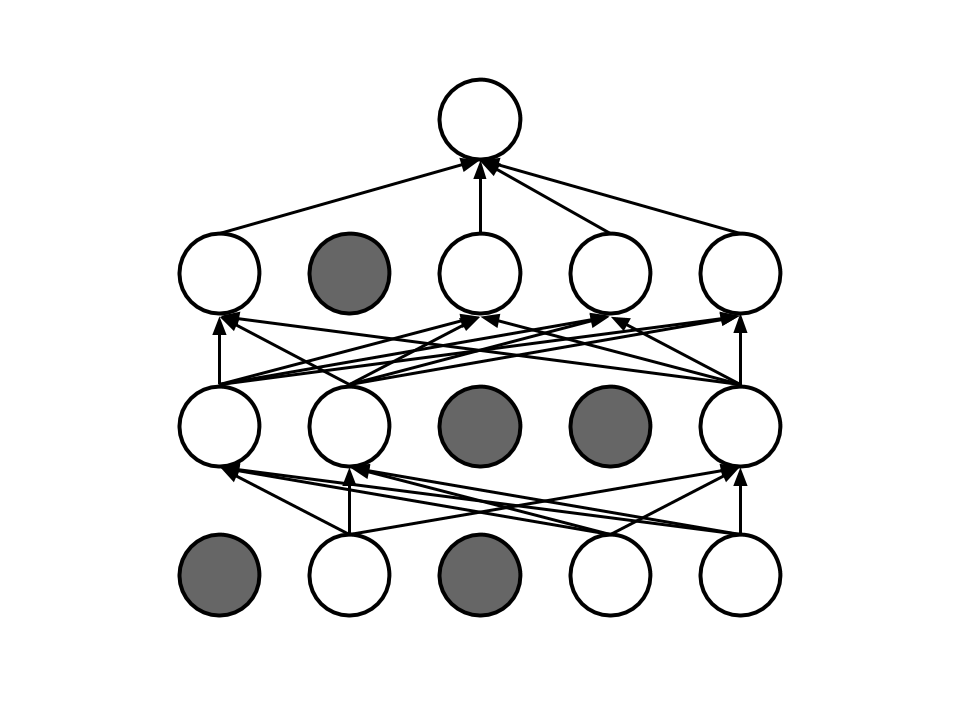
\includegraphics[scale=0.15]{images/chap2_dropout_b.png}\label{fig:chap2_dropout_b}}
\subfloat[][隨機丟棄部份神經元的DNN]{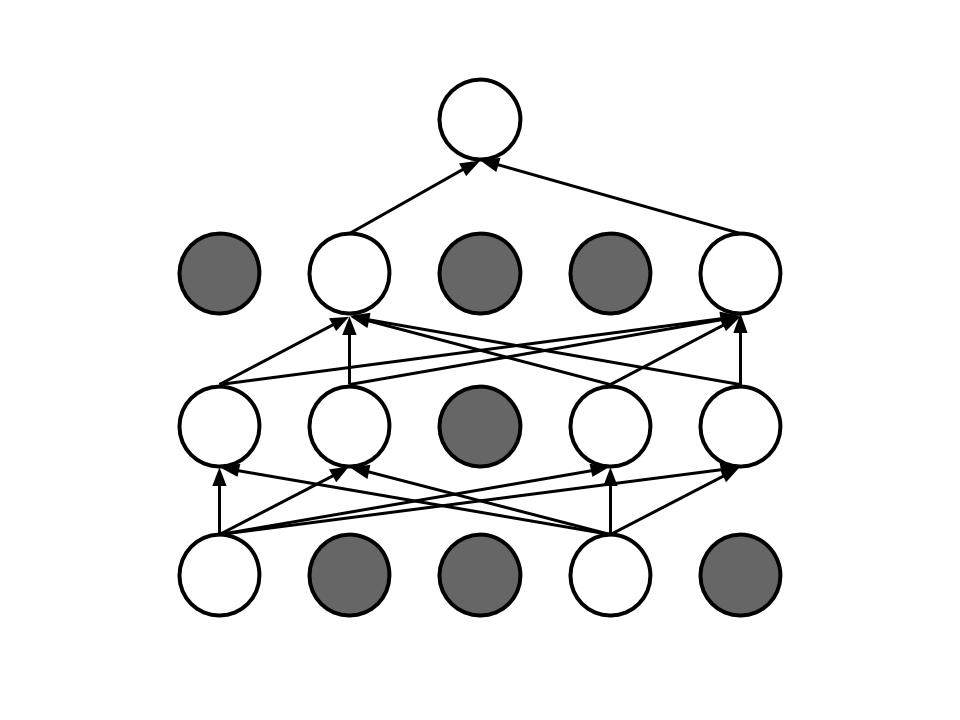
\includegraphics[scale=0.15]{images/chap2_dropout_c.png}\label{fig:chap2_dropout_c}}
\caption{丟棄演算法示意圖。其中(b)與(c)是兩種不同的丟棄配置,因為隨機性而有了多樣化,分別是較小的模型,但整合成一個比(a)來得強大的整合模型。}
\end{figure}

丟棄演算法同時也可以視為隨機整合(Random Ensemble)模型。整合模型(Ensemble Model)在機器學習領域已經被證明是非常強大的模型,藉由多個模型的多樣性(Diversity)各司其職,提昇模型強度。類比在丟棄演算法中,根據不同的丟棄情況,有不同的神經元組合互相整合而成。隨機性造就了多樣性,又同時控制調適,使得模型更不容易過度適應。
\section{全球音素語料庫(GlobalPhone Corpus)}
\subsection{語料介紹}
全球音素語料庫(GlobalPhone Corpus, GP)是德國卡斯魯爾大學(Karlsrusher University, 現在卡斯魯爾理工學院前身)的譚雅.修姿女士(Tanja Schultz)所主持、設計與收集的多語言語料庫,專門設計給語音辨識系統發展與研究使用。語料庫內含15種語言,每種語言也有80位以上的語者變化,使得語料庫總計有300小時以上的聲音檔,1500位以上的在地成人語者聲音資料庫。不同語言間的錄製環境、設計準則皆一致,唯有語言和語者的差異,以方便進行跨語言的系統設計與實驗比較。

GP發展之初,是為了研究獨立於語言之間的全球音素集(Global Phone Set),以輔助相依於不同語言的的辨識系統,從其全球音素之命名可見一斑。語言學家對於多語言辨識系統具有高度興趣,需要品質較好、設計準則一致又富含多樣化語言的語料庫,這樣的需求顯然催生了GP。然而世界語言已經超過4500種,GP在挑選語言上亦費了一番功夫。為了挑選最能代表世界語言的組合,GP至少考量了:
\begin{itemize}
\itemsep -2pt 
 \item 語者數量
 \item 語者政治跟經濟環境多樣性
 \item 地理範圍(然非洲因無穩定經濟體系,語料收集困難,語系亦複雜多變,故無考慮非洲)
 \item 語言包含的音素範圍
 \item 語系和語形分佈。
\end{itemize}
GP先於當時的國內外報章雜誌中蒐集政經相關文字,由指定語者唸出文字錄製而成,是為閱讀型語音(Read Speech)。所有的語音都在一兩年內錄製完成,確保每個語言之間共通名字(如政治家、都市、公司)的一致性。這些錄音檔都經過人工的二次確認,包含斷句、發音錯誤等等。除了聲音所對應的文字以外,亦額外收集大量的文字資料。這些資料並不額外錄音,僅供訓練語言模型。


本論文選擇了GP四個印歐語系語言,分別為西斯拉夫語支的捷克語(Czech, CZ)、西德語支的德語(German, GE)、西伊比利亞語支的西班牙文(Spanish, SP)、和高盧羅曼語支的法文(French, FR)。這四個語言的基本資料如附錄。
\subsection{國際音標(International Phonetic Alphabet, IPA)}
國際音標是語言學家為了更有效率表達世界上各種語音而設計的一套符號規則。最早由國際語音學學會(International Phonetic Association)所建,而後修改擴充,以清楚描述世界上任何人類語音的聲音。

針對任一語言,國際語音學學會會針對其中的每一個可鑑別音(Distinctive Sound),進行音素轉寫(Phonetic Transcription),對應到國際音標上的一種獨立符號。即便物理上兩者呈現不同的聲音,但如果在該語音母語人士人耳中無法鑑別,則必須被標記為同一種音素(Phone)。因此,一種語言通常只會用到部份的國際音標。

國際音標中最常使用的通常為母音(Vowel)與子音(Consonant)的部份,合稱肺部氣流音(Pulmonic)。母音在國際音標中,以母音四邊型(Vowel Quadrilateral)的方式呈現,如圖\ref{fig:vowel};子音則為一張藉由發音方式以及發音位置交錯整理而成的表格,如圖\ref{fig:consonant}。

\begin{figure}
\centering
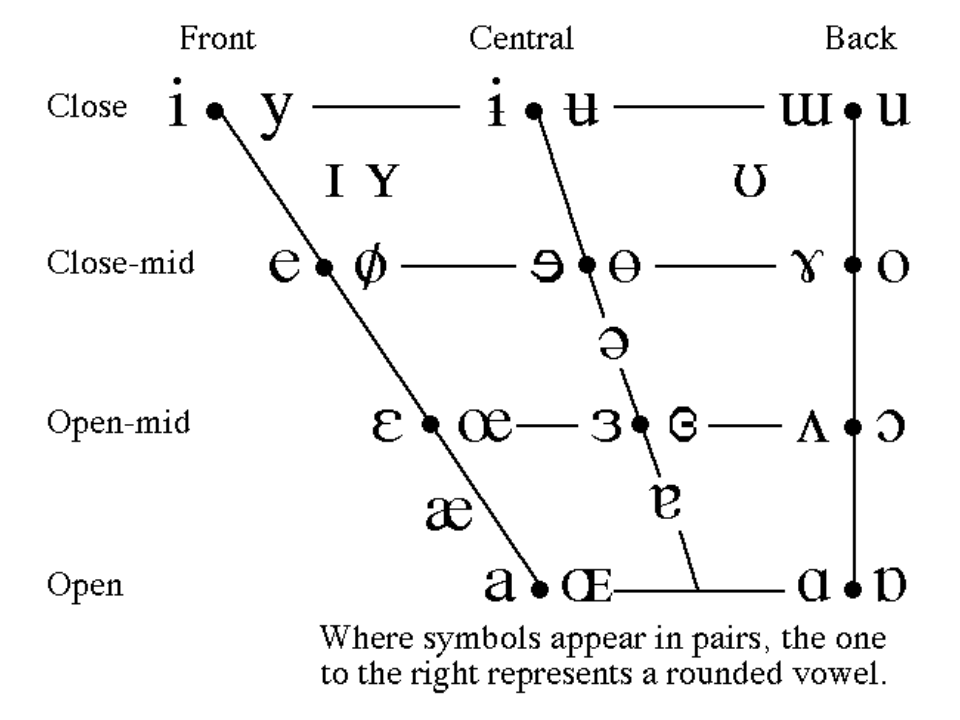
\includegraphics[scale=0.4]{images/chap2_vowel_quadrilateral.png}
\caption{母音四邊形}
\label{fig:vowel}
\end{figure}

\begin{figure}
\centering
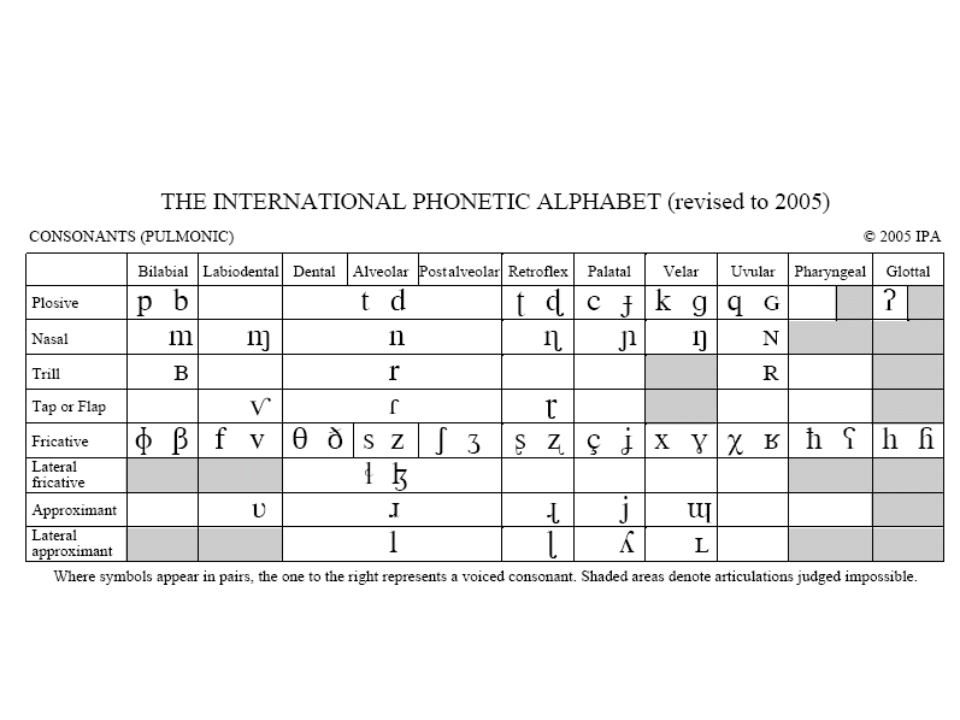
\includegraphics[scale=0.4]{images/chap2_consonant.png}
\caption{子音表}
\label{fig:consonant}
\end{figure}
母音四邊形類比於人類口腔,每一點代表發音時,舌頭在口腔中的接觸位置。左右代表口腔前後,上下亦然。同一位置上如有兩種音素,右音素為圓唇音(Rounded),一如其名,發音時須圓唇。

子音表格中,左邊根據不同發音方式分類,上邊根據不同發音接觸位置分類。同一位置上如有兩種音素,右音素為聲帶靠近時發出的濁音(Voiced),左音素則為聲帶遠離時發出的清音(Unvoiced)。有些格子為灰色,代表人類不可能發出的發音組合。

一般而言,子音與母音已經能夠廣義地涵蓋所有發音單位。然各語言有其特色,往往需要額外地在廣義轉寫符號上標記各種程度的細節,形成讀音符號(Diacritic)。本論文所選的四種語言,除了其原生的音素以外,亦標記了各個音素對應的國際音標表於附錄。

\section{多語言語音辨識系統}
多語言語音辨識系統的發展,有各種不同的情景,相關的研究亦有不同的靈感、切入點以及評估方式:
\subsection{語言混合(Code-Mixing)}
有些地區的人民,可能因為科技發展、地緣關係的因素,同時熟稔兩種以上的語言,其熟稔程度除了單純的句子交錯、名詞抽換之外,甚至有可能文法參雜,借用別的語言的句式。這些語言混合(Code-Mixing, CM)的核心問題,在於如何準確找到語者切換不同語言時的切換點(Code-Switching Point, CS Point)。如圖\ref{fig:chap2_cs}。

語言混合的例子,隨著時代變遷越來越明顯,如:
\begin{itemize}
\itemsep -2pt
\item 歐盟(European Union, EU)裡每個成員都具備至少三種語言的隨時切換能力,常會有一個人以德文發問、另一人以西文回答、第三人用德文混法文補充。
\item 亞洲的教育體系往往保留原文的發音與字詞,如在中文的文法裡中加入英文的專有名詞。
\end{itemize}
語言混合的問題,通常會將語言分為基質語言(Matrix Language)與嵌入語言(Embedded Language),這樣的分類主要根據混合比例。基質語言通常是語者的原生語言,決定該句子的文法句式和主要發音音素。嵌入語言則為客串,若基質語言無法呈現某些關鍵意涵時,語者可能轉而使用嵌入語言表達。然基質語言和嵌入語言的比例不均,在訓練語音辨識系統時,造成系統偏好資料量較多的基質語言,而無法成功辨識資料量較少的嵌入語言。

為了解決資料量不足的問題,可以將基質語言和嵌入語言中近似的發音單位合併訓練。合併單位可能從較高層級的音素層級、越發細緻到更底層的三連音態(Triphone state, or Senone)層級,如圖\ref{fig:chap2_merge}。
\begin{figure}
\centering
\subfloat[][語言混合資料示例,黃線為語言切換點]{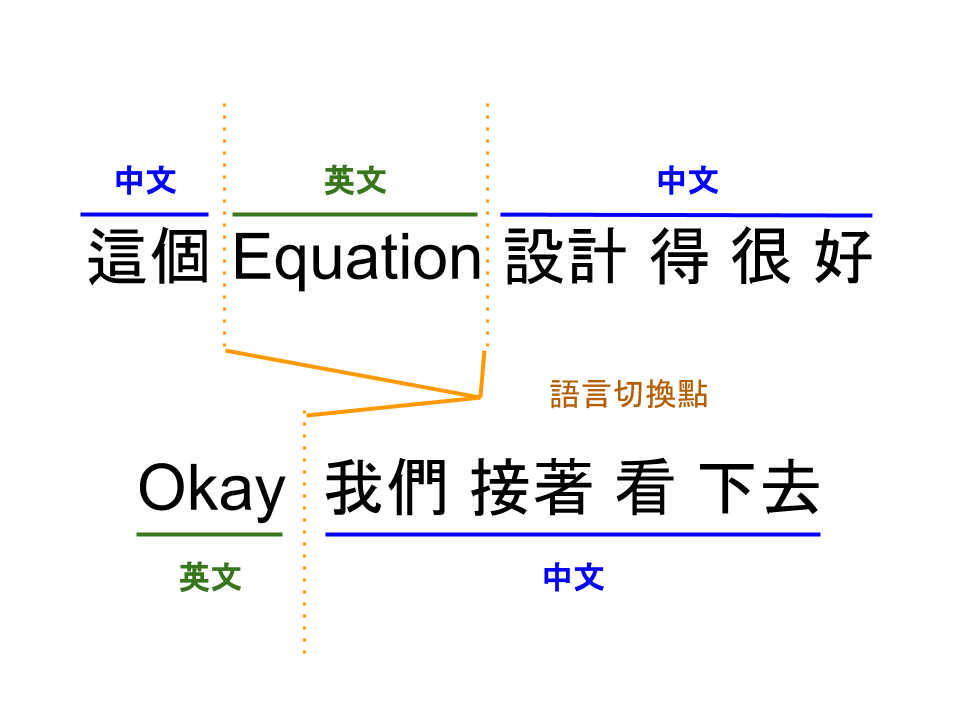
\includegraphics[scale=0.25]{images/chap2_cs.png}\label{fig:chap2_cs}}
\subfloat[][三連音態合併的深層類神經網路訓練]{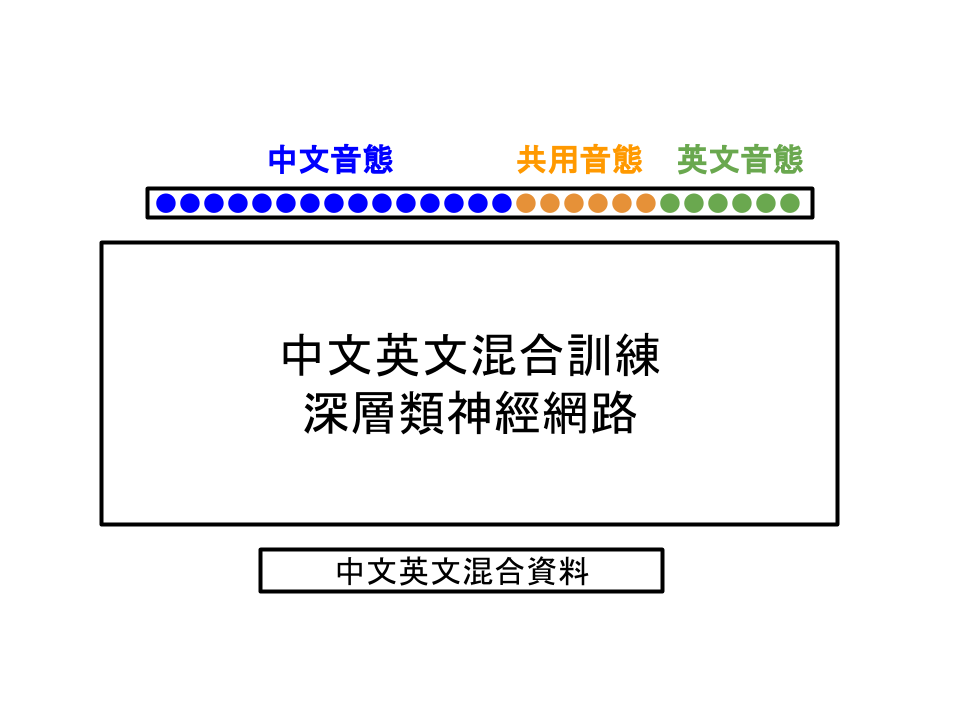
\includegraphics[scale=0.25]{images/chap2_merge.png}\label{fig:chap2_merge}}
\caption{以中文混合英文的語言混合問題與模型訓練方法。}
\end{figure}
%因應比例不同,亦可以先訓練嵌入語言偵測器,當偵測器發現時嵌入語言時,將嵌入語言的事後機率拉高,形成模糊化事後機率特徵(Blurred Posteriorgram Features, BPFs)。

在評估語言混合問題時,除了兩種語言的結果都必須分別分析之外,因為嵌入語言的數量較少,討論時往往深入探討嵌入語言的辨識率。


\subsection{跨語言轉移學習(Crosslingual Transfer Learning)}
跨語言轉移學習是借助豐富大量的來源語言(Source Languages),以幫助資源稀少(Low-resourced)的目標語言(Target Language)訓練語音辨識系統。當資料量過少的時候,一般的機器學習方法就容易陷入瓶頸,遑論亟需資料量的深度學習。
例如非洲、東亞戰亂地區的語言。這些語言本身收集困難,又因為軍事政治環境的關係,有語音辨識或是關鍵字擷取(Keyterm Extraction)的需求。軍方有可能採集少量的該地聲音作為目標語言。相比之下,GP的資料量非常豐富,也非常乾淨,與資源稀少的語言相當不匹配。

語言間或多或少有共通的聲音特色,常見的轉移學習便是以大量豐富資料前置訓練(Pretraining)一個來源語言的語音辨識系統,再以目標語言的少量資料微調(Fine-tune)成目標語言的語音辨識系統,如圖\ref{fig:chap2_cross}。

\begin{figure}
\centering
\subfloat[][以來源語言訓練]{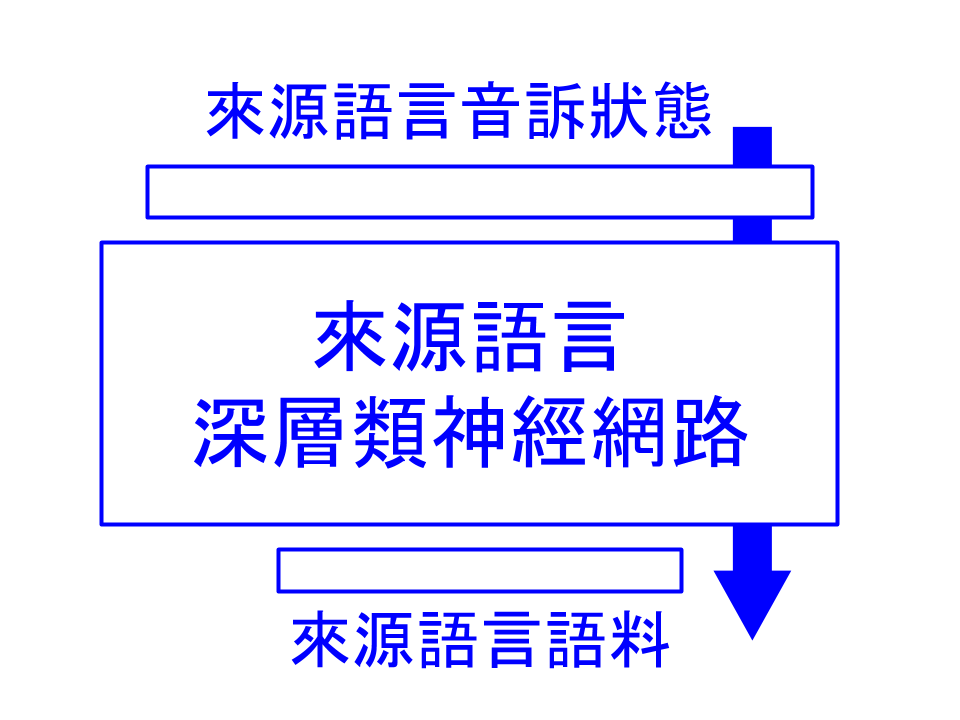
\includegraphics[scale=0.15]{images/chap2_cross_source.png}\label{fig:chap2_cross_source}}
\subfloat[][以目標語言微調]{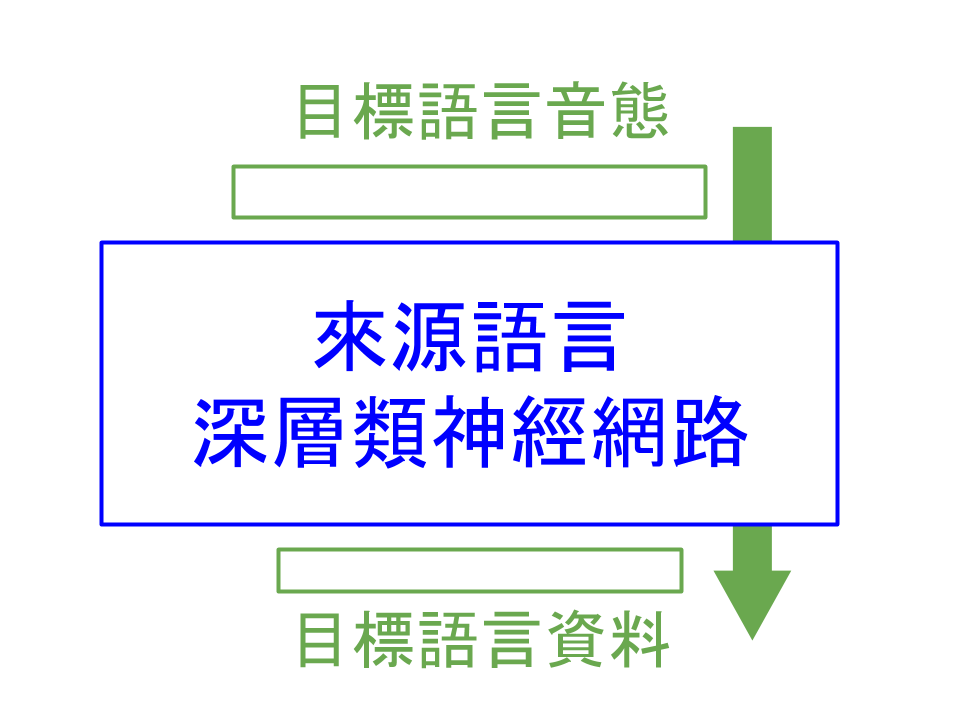
\includegraphics[scale=0.15]{images/chap2_cross_target.png}\label{fig:chap2_cross_target}}
\subfloat[][微調後模型同時包含兩者資訊]{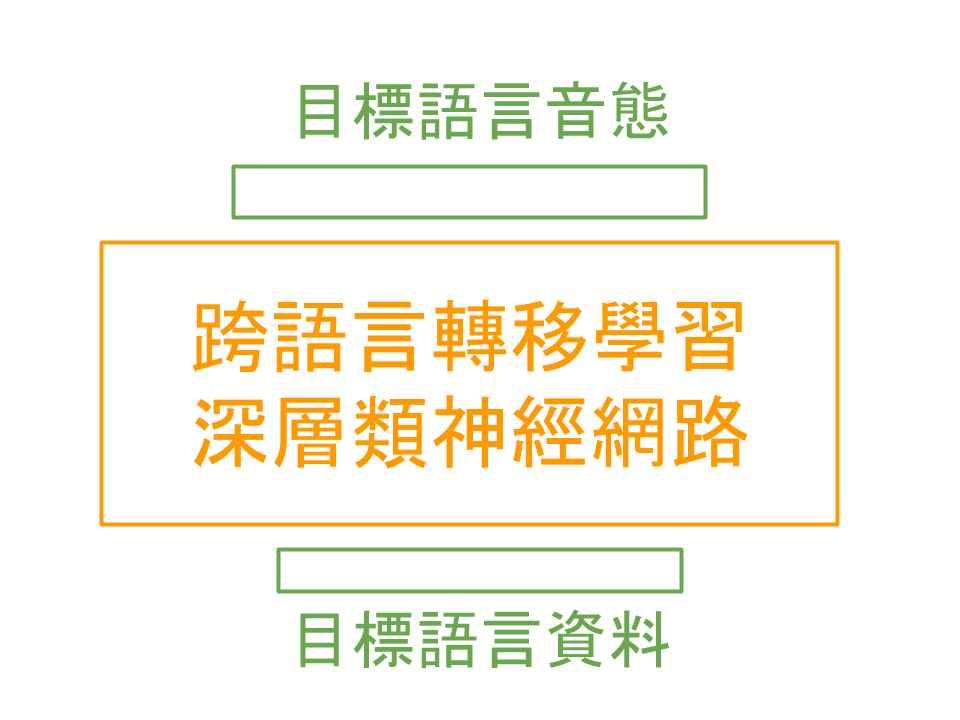
\includegraphics[scale=0.15]{images/chap2_cross_finetune.png}\label{fig:chap2_cross_finetune}}
\caption{訓練跨語言轉移學習類神經網路,由左至右依序訓練,箭頭則是訓練時從輸出反向傳播至輸入的方向。}
\label{fig:chap2_cross}
\end{figure}


\subsection{多語言共享學習(Multilingual Sharing)}
結合上述的情景,多語言語音辨識系統的關鍵,便是能否在多如繁星的各種語言中,找尋共通的資訊,彼此輔助學習。一來減少對單一語言的資料量依賴性,二來可以提供更多語言的語音辨識系統,如圖\ref{fig:chap2_multilingual}。這包含了許多種不同層級的共享,像是語言混合問題中提到的發音單位共享,或是跨語言轉移學習中提到的模型微調。

但這個問題並不像語言混合一樣針對嵌入語言,也不似跨語言轉移學習問題中一樣針對目標語言。多語言共享學習希望能找出不同語言中的共享精華,例如全球音素集,或是更細緻的全球音態集(Global Senone Set),因而對待每個語言的比重平等,旨在希望不同語言間的資訊可以互惠,而不是單方面的施與受。在評估表現時,須特別注意多個語言表現的整體性,以免顧此失彼。

\begin{figure}
\centering
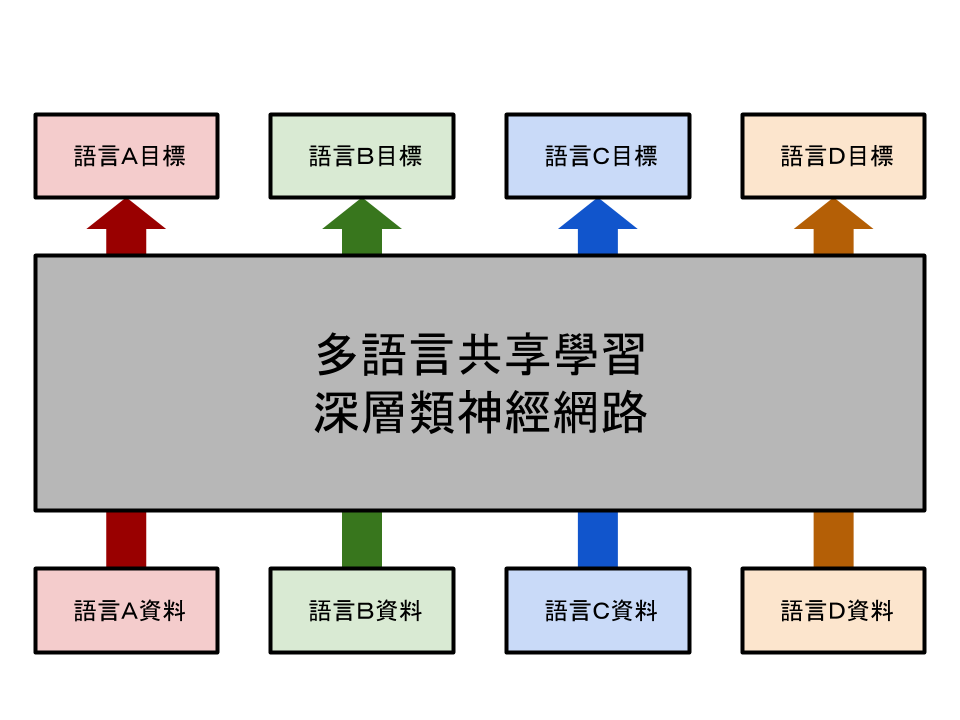
\includegraphics[scale=0.4]{images/chap2_multilingual}
\caption{多語言共享學習,四個語言各自獨立評估卻又相輔相成,互相學習。}
\label{fig:chap2_multilingual}
\end{figure}

\chapter{單語言基礎實驗}
  \section{單語言語音辨識系統架構}
在了解多語言辨識系統之前,必須先設計好一個足夠強大的單語言語音辨識系統,以深入且正確地探討多語言情景下的資訊。本論文所使用的單語言辨識系統架構如圖\ref{fig:chap3_framework}。
\begin{figure}[!h]
\centering
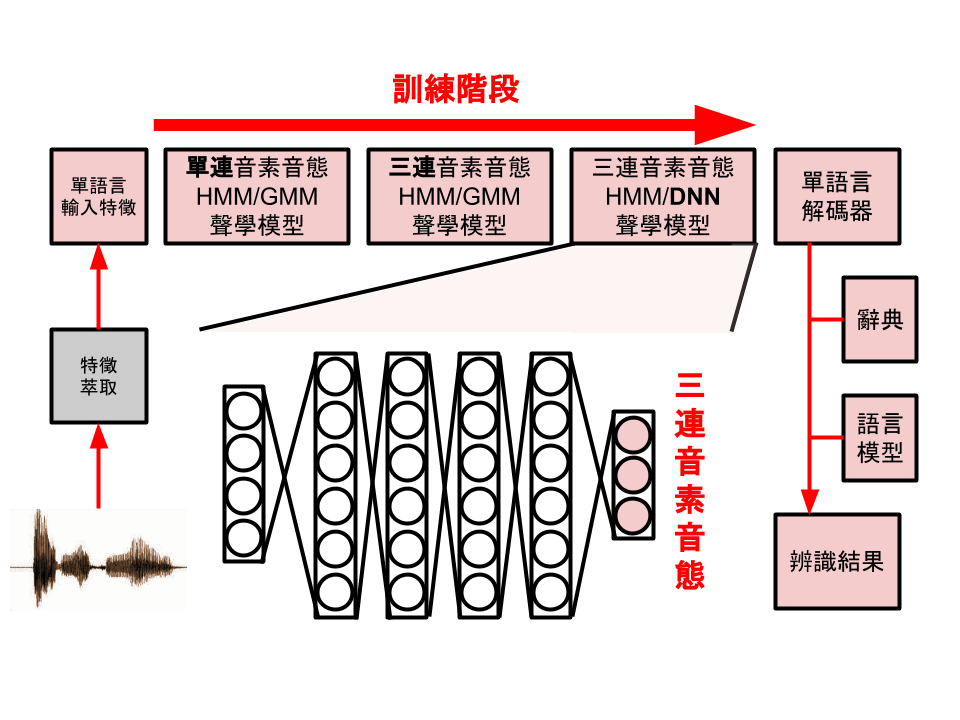
\includegraphics[scale=0.4]{images/chap3_framework.png}
\caption{單語言語音辨識統架構圖}
\label{fig:chap3_framework}
\end{figure}

本論文使用GP中的四個語言(西班牙語SP,捷克語CZ,法語FR,德語GE)做為實驗語料,因此會訓練出如圖\ref{fig:chap3_monolingual},四個互相獨立的單語言辨識系統,各自在自己的語言上辨識並回報結果。

四個語言分別有自己的訓練集(Training set)、發展集(Development set)以及測試集(Test set),由GP官方以8:1:1的比例設計,詳細數據請參考附錄。

\begin{figure}[!h]
\centering
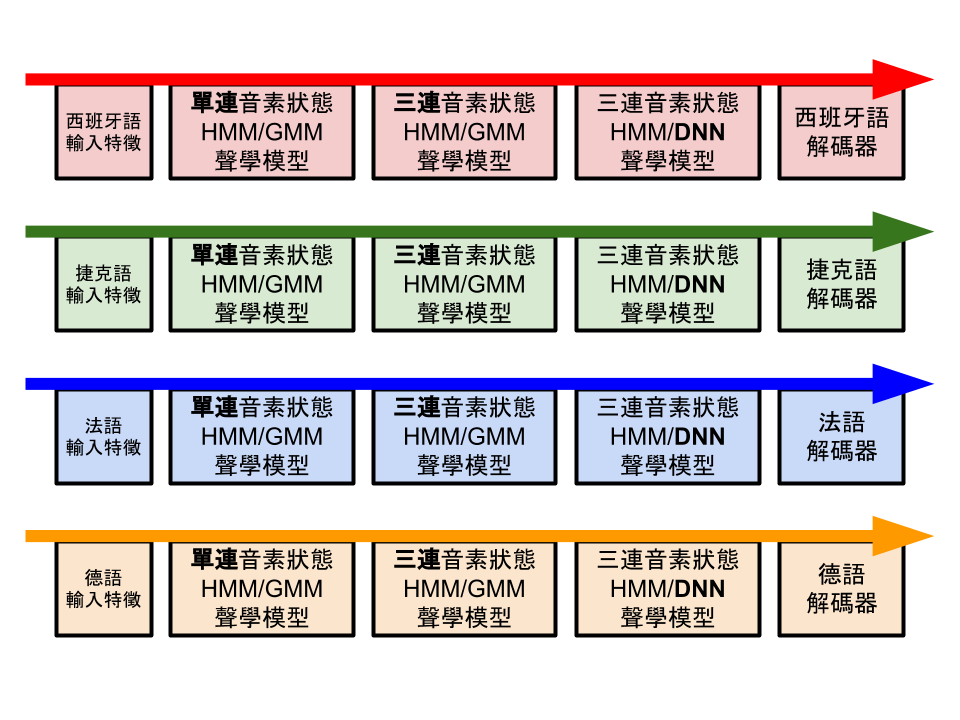
\includegraphics[scale=0.4]{images/chap3_monolingual.png}
\caption{西班牙語、捷克語、法語、德語的單語音辨識系統}
\label{fig:chap3_monolingual}
\end{figure}
\subsection{特徵萃取(Feature Extraction)}
給定麥克風收入的語音電訊號,特徵萃取旨在將此時頻訊號,轉換成更富含語言意義且較低雜訊的特徵向量,做為下一階段聲學模型的輸入。

特徵萃取階段,會從聲音訊號中取出寬度25毫秒的音框(Frame)。針對一句話連續取樣音框時,音框中心點間隔10毫秒,因此必然有重疊部分,以降低邊界雜訊。每個音框內計算訊號的梅爾頻率濾波組(Mel-frequency Filterbanks, FBANK),取其不包含能量(Energy)的23維頻率強度。一個音框為模型的一筆訓練實例(Training Instance)。

這23維特徵,會經過一階差分以及二階差分,計算出總計69維的輸入特徵。接著經過語者譜頻平均正規化(Speaker-wise Ceptral Mean Normalization, CMN),分別調整各維度的值,使得同樣語者分佈在不同句子的所有訓練實例中,同維度的平均值皆為0。正規化能夠一定程度地降噪,同時能有效降低語者之間的差異性,使得不同語者的聲音都能轉換在共同的輸入空間上設計系統。

然語音乃高度結構化的訊號,訓練深層類神經網路的時候,還會把單一音框和前後文(Context)音框同時黏合起來。以前四後四為例,對每一個訓練實例,把前後各四個音框的向量與之結合,形成總共$69 \times (4 + 1 + 4) = 621$維的輸入向量。前後文相依(Context-dependent, CD)提供更強大的預測能力,對於深層類神經網路的模型訓練複雜度幾乎沒有影響,卻對高斯混合模型造成強大的訓練時間懲罰。

\subsection{聲學模型(Acoustic Modeling)}
給定萃取後的特徵向量序列,聲學模型旨在將此序列轉換成對應的發音單位序列,經過辭典(Lexicon)轉換成有文字意義的詞彙序列,做為下一個階段語言模型的輸入。

聲學模型乃利用數學模型得到以下的機率:
\begin{equation}\label{eq:am}
p( \bold{s} | \bold{x}_1 , \bold{x}_2 , ... , \bold{x}_T ) = \frac{ p( \bold{x}_1 , ... , \bold{x}_T | \bold{s} )p( \bold{s} )}{ p( \bold{x}_1 , \bold{x}_2 , ... , \bold{x}_T ) }
\end{equation}

其中$\bold{s} = \{s_1 , s_2 , ... , s_T \}$是發音單位的序列,$\bold{x}_t$為輸入的第$t$個音框特徵向量,一句話總計有$T$個音框。

公式\ref{eq:am}根據貝式定理(Bayes Theorem),針對整句話的發音單位建模。因此,整個模型拆解成兩個部分,一個為發音單位之間變化的轉移模型(Transition Model)如公式\ref{eq:am_trans}。
\begin{equation}\label{eq:am_trans}
p( \bold{s}) = p(s_1)\prod_{i=2}^{T} { p( s_i | s_{i-1} ) } 
\end{equation}

以及單音框內發音單位與特徵向量的分布模型(Emission Model),如公式\ref{eq:am_emit}。

\begin{equation}\label{eq:am_emit}
p( \bold{x}_1 , \bold{x}_2 , ... , \bold{x}_T | \bold{s} ) = \prod_{i = 1}^{T} p( \bold{x}_i | s_i )
\end{equation}

使用聲學模型時,旨在找到最可能的發音單位序列能夠最大化這個機率:
\begin{equation}\label{eq:am_argmax}
 \bold{s}^* =  \arg\max_{\bold{s} } \frac{ p( \bold{x}_1 , ... , \bold{x}_T | \bold{s} ) p( \bold{s} ) } { p( \bold{x}_1 , \bold{x}_2 , ... , \bold{x}_T ) } = \arg\max_{\bold{s} }  p( \bold{x}_1 , ... , \bold{x}_T  | \bold{s} ) p( \bold{s} ) 
\end{equation}

其中轉移模型利用馬克夫鏈(Markov Chain)的概念,將每一個發音單位的分布機率限定在只根據前一個發音單位。分布模型則把每一個音框的相依性拆開,使得整個序列的分布機率僅為個別音框的分布機率乘積。

在替分布模型建模的時候,最原始的作法是使用高斯混和模型(Gaussian Mixture Model, GMM),替每一個發音單位,用一把不同權重的高斯分布加權總合計算出機率。因為以高斯函數計算機率的運算複雜度受維度大小影響甚大,為了保持可接受的運算時間,通常僅根據於69維的FBANK特徵建模。

進階的分布模型建模時,可以將原本替個別音框分布機率的公式\ref{eq:am_emit},再度以貝式定理拆開,如下:
\begin{equation}\label{eq:am_emit_framewise}
p( \bold{x}_i | s_i ) = \frac{ p( s_i | \bold{x}_i) p( \bold{x}_i ) } { p ( s_i )}
\end{equation}

其中$p(\bold{x}_i )$會在使用聲學模型時,如同公式\ref{eq:am_argmax}時一樣捨棄掉。$p( s_i )$為該發音單位的事前機率,可以藉由統計所有音框的發音單位來獲得。$p( s_i | \bold{x}_i )$為一個分類器問題,給定輸入特徵向量$\bold{x}_i$,分類為發音單位$s_i$的機率,可以使用深層類神經網路來建模,以及$621$維的高維度輸入特徵,以達到更好的預測準確率。

在替轉移模型建模時,必須先決定好建模所使用的發音單位。語言學家定義音素(Phone)為人耳可鑑別的最小發音單位,然對於機器而言,音素的層級太過粗糙,無法囊括聲音訊號的變化。最原始的做法是使用隱藏式馬可夫模型(Hidden Markon Model, HMM)作為轉移模型,將每一個音素拆解成三種發音狀態,稱為單連音素音態(Monophone state)。

然以單連音素音態作為發音單位仍然不夠細緻,因為音素在不同的前後文(Context)中,依然有不同的特徵表現。因此,考慮三個連續音素的組合變化,把一組三連音態用三種發音狀態拆解,稱為三連音素音態(Triphone state)。因為音素約莫40個,三連音態的組合便有$40^3 \times 3= 192000$種三連音素音態。這個輸出維度太過龐大,某些組合的資料量太小,因此有些相近的三連音素音態會合併起來視為同一種發音單位。

整個聲學模型的訓練過程,就是一種由淺入深的過程。萃取好特徵向量之後,一步一步將發音單位磨得越來越細緻。回顧圖\ref{fig:chap3_framework},一開始建立HMM與GMM的單連音素音態模型,然後拆解成三連音素音態的模型,最後把高斯混合模型切換成深層類神經網路,重新建模。

有了聲學模型,利用公式\ref{eq:am_argmax}能夠找出最好的發音單位序列,搭配辭典,可以將發音單位序列組合成字或詞的序列。實務上,聲學模型會保留機率夠高的多組序列輸出,以免因為模型誤差把可能的正確序列提早屏除掉了。

\subsection{語言模型(Language Modeling)}

給定聲學模型篩選出的字詞序列,語言模型可以根據字詞之間的意義相關性與文法合理,給予語言知識上的評分。

給定詞序列,語言模型在於估計以下機率:
\begin{equation}
p( w_1 , w_2 , w_3 , ... , w_L )
\end{equation}
其中L為該序列對應的詞的數量,$w_i$為序列中的詞。

一般而言,常用多連文法(N-gram)來建模:
\begin{equation}
p( w_1 , w_2 , w_3 , ... , w_L ) = \prod_{i = 1}^L p( w_i | w_{i-1} , w_{i-2} , ... , w_{i-N+1} )
\end{equation}

N的決定來自於系統規模的考量。產品設計上可能會到4,5甚至6,研究上取N=3,三連文法即足夠。

由於語言模型是跳脫於語音文件外的,因此通常可以採用額外的巨量數據來補足,形成背景模型(Background Model)。如果語音辨識時能夠知道文字的特定領域,例如是否屬於報章雜誌?還是科技期刊?或是網路討論?情感抒發?不一樣的文字內容,亦可能需要不同的語言模型來建模。這些針對的領域模型(In-domain Model),還可以與背景模型加權平均,形成內插模型(Interpolation Model)。內插模型能夠提供背景模型的強大力量,又能針對領域與特定知識提供分數,往往擁有較好的表現。

\subsection{解碼器(Decoder)}
有了聲學模型、語言模型,解碼器旨在把所有的模型統合起來,形成一個由聲音訊號到文字序列的辨識系統。

理論上,聲學模型、辭典、語言模型是三個輸入與輸出剛好匹配的系統,能夠一直線到底完成系統。實務上,為了整體系統設計更為穩健,避免前端系統的錯誤提早刪去正確序列,解碼器的演算法設計除了著重時間、空間複雜度之外,還須考量模型的彈性。這包含:

\begin{itemize}
\itemsep -2pt %reduce space between items
  \item 語音辨識是在整個輸入向量空間中,樹狀搜尋分數最高的一條路線。然樹狀分支會隨著解碼序列增長而變得龐大,因此必須進行光束刪減(Beam Pruning),在某時刻只保留部份最具可能性的序列,傳遞至下一階段。這個保留的比例是系統設計的一個彈性參數,保留越少越需要的解碼時間越短,但卻可能提早把正確序列捨棄掉。

 \item 語音辨識中,聲學模型與語言模型各自佔有不同的地位。前者試著保留聲音以及發音單位的關聯性,後者則估計不同字詞間相連的合理性。這兩者的權重比例是解碼器設計的一個彈性。前者的比例越高,表示系統越重視聲學模型所訓練出來的聲音,但卻可能讓出來的文字序列意義不彰。

 \item 語音辨識系統由許多不同的子系統組合而成,各自蓬勃發展,系統必須要支援各個子系統的熱插拔(Plug and Play, PnP),能夠彈性地切換不同的聲學模型、語言模型以及辭典。
\end{itemize}

現在的語音辨識解碼器演算法,通常根據於加權有限狀態傳感器(Weighted Finite State Transducer, WFST),將不同的模型轉換成WFST的格式儲存在電腦或是雲端的記憶體裡。如:



\begin{table}[htbp]
%\resizebox{\columnwidth}{!}{
\centering
\begin{tabular}{|cccl|}
\hline
 代號 & 輸入 & 輸出 & 備註 \\
\hline
 U    & 三連音素音態 & 三連音素音態 & 權重為聲學模型分佈機率 \\
\hline
 H    & 三連音素音態 & 三連音素音態 & 權重為聲學模型轉移機率 \\
\hline 
 C    & 三連音素音態 & 音素 & 無權重  \\
\hline
 L    & 音素 & 詞 & 無權重,由辭典產生,將可能的音素對應回詞 \\
\hline
 G    & 詞 & 詞 & 權重為語言模型詞序機率   \\
\hline

\end{tabular}
\caption{解碼器相關WFST的輸入輸出與權重意義}
\label{table:chap3_wfst}
\end{table}

語音辨識模型中,聲學模型、辭典以及語言模型能夠分別轉換化成對應的H、C、L、G,並且組合(Composition)成一個統一的WFST,合稱HCLG,是辨識系統的核心本體。每當一段聲音訊號進入,系統會先進行特徵萃取,將萃取好的特徵向量序列,輸入訓練好的深層類神經模型,產生出一個句子的WFST,為表\ref{table:chap3_wfst}中的U。

U會與記憶體裡的HCLG再度組合(Composition),形成U-HCLG。組合過程中的U-HCLG佔據非常大的記憶體,因此在組合過程中便會進行光束刪減(Beam Pruning)。組合完畢的U-HCLG再經由WFST的最短路徑(Shortest-path)演算法,找到分數最高的一條路徑,將路徑上的詞序全部輸出,即為辨識結果。辨識結果與語料庫提供的正確詞序比較,得到詞誤率(Word Error Rate, WER),作為評估的考量。詞誤率是評估語音辨識最重要的參數之一,越低代表著辨識系統錯誤的詞越少。

研究上,聲學模型的訓練過程,以及解碼器的諸多彈性參數,都必須根據情景調整,沒有一個通用的最佳解。學術上的慣例會以語料庫中的訓練集作為訓練模型的資料,而以發展集作為調整解碼器的參數,如光束大小、語言模型的權重等等。
\section{深層類神經網路基礎實驗設計}
本論文評估單語言語音辨識系統的基礎實驗設計,旨在探討語言模型、丟棄演算法、深層類神經網路的參數設定,作為之後多語言語音辨識系統的基準實驗。
\subsection{語言模型}
評估語言模型的方式有兩種方式,一種為混淆度(Perplexity),用以衡量語言模型於給定測試語料的分數,公式如下:
\begin{equation}
PPL(w_1 , w_2 , w_3 , ... , w_L ) =  p(w_1 , w_2 , w_3 , ... , w_L ) ^{-\frac{1}{L}}
\end{equation}
混淆度越大,表示語言模型在預測該文字測試語料的信心指數越低。

% TODO REF SRILM
評估單語言語音辨識系統之前,本論文使用三種不同的語言模型,分別針對GP的純文字測試語料計算混淆度。三種模型分別為:

\begin{table}[htbp]
%\resizebox{\columnwidth}{!}{
\centering
\begin{tabular}{|c>{\columncolor{red!20}}c>{\columncolor{green!20}}c>{\columncolor{blue!20}}c>{\columncolor{yellow!20}}cc|}
\hline
 模型名稱 & 西班牙語 & 捷克語 & 法語  & 德語 & 備註 \\
\hline
 背景模型 & 1.40M    &  1.05G & 85.3M & 66.9M & GP官方提供的語言模型 \\
\hline
 領域模型 & 2.74M    &  3.57M & 4.08M & 3.73M & 使用GP訓練語料文字訓練而成 \\
\hline
 內插模型 & 3.15M    &  468M  & 87.1M & 67.2M & 等比例內插背景模型以及領域模型 \\
\hline
\end{tabular}
\caption{四個語言分別三種不同語言模型的模型大小。官方提供的西班牙語語言模型規模小,嚴格來說不像是背景模型。捷克語的內插模型過大,因此有使用辭典刪減不在訓練集內的詞的參數。}
\label{table:chap3_lm_stat}
\end{table}


三個模型除了混淆度之外,亦會與深層類神經網路的聲學模型結合,計算詞誤率,結果如表\ref{table:chap3_lm}。



\begin{table}[htbp]
%\resizebox{\columnwidth}{!}{
\centering
\begin{tabular}{|cc>{\columncolor{red!20}}c>{\columncolor{green!20}}c>{\columncolor{blue!20}}c>{\columncolor{yellow!20}}c|}
\hline
 語言模型 & 評估指數 & 西班牙語 & 捷克語 & 法語 & 德語 \\
\hline
 \multirow{2}{*}{背景模型}&      PPL & \underline{161} & 1421 & 357 & 680 \\
        &      WER & \underline{8.68\% } & \underline{18.13\% } & 20.87\% & 17.85\% \\
\hline
 \multirow{2}{*}{領域模型}&      PPL & 284 & \underline{1076} & \underline{275} & 934 \\
        &      WER & 23.76\% & 43.19\% & 22.86\% & 19.51\% \\
\hline
 \multirow{2}{*}{內插模型}&      PPL & 206 & 1317 & \underline{284} & \underline{641} \\
        &      WER & 10.34\%  & 20.12\%  & \underline{17.21\%} & \underline{15.28\%} \\
\hline
 官方數據 &      WER & 10\%  & 15.7\%  & 19.5\% & 14.2\% \\
\hline
\end{tabular}
\caption{四個語言的單語言辨識系統在不同語言模型下的詞誤率,包含語言模型在相應的測試集計算而得的混淆度。表中的詞誤率計算,都是使用4層寬度為2048神經元並使用S型函數作為活化函數的深層類神經網路聲學模型。}
\label{table:chap3_lm}
\end{table}

從表\ref{table:chap3_lm}可以看到混淆度與詞誤率有一定程度的正相關,混淆度越低通常意味著詞誤率越低。然在計算詞彙外(Out-of-Vocabulary, OOV)的詞時,混淆度會直接跳過不納入考量,而詞誤率則會直接反應在數據上。即便捷克語以及法語的領域模型混淆度都較低,該語言模型在詞誤率的表現卻很差,因為領域模型的訓練資料只有GP的訓練集的句子,資料相比背景模型而言少非常多。

內插模型擁有領域模型的豐富資訊,和領域模型的特定資訊,因此在法語跟德語上表現結果較好。西班牙語跟捷克語的訓練集較不匹配測試集,使用背景模型本身比較好,加入領域模型沒有提供更多資訊。

之後的實驗針對不同語言,解碼器所使用的語言模型,為本表格中測試詞誤率最低的相應語言模型。然而,這個行為違反了機器學習的驗證理論,理論上不應該從測試集的結果中進行挑選。但本研究核心內容著重在聲學模型的設計與實驗比較,為了建立較強力的基準實驗系統,特意揀選語言模型。之後實驗亦不再多做討論語言,僅在此呈現數據。


\subsection{丟棄演算法}
深層類神經網路深受過度貼合的影響,丟棄演算法是典型的控制適應來避免過度貼合。然丟棄演算法的隨機性會破壞訓練的穩定度,在過程中強制關閉神經元輸出,會丟棄神經網路學到的資訊。一般而言,語音訊號的丟棄比例設定在$0.05 - 0.1(5\% - 10\%)$之間。本實驗的丟棄比例為0.1,即10\%。

一般的類神經網路會使用S型函數作為活化函數。S型函數在接近0的位置變化量最大,因此能夠拉開神經元在接近閾值時的些微變化,讓神經網路對於細微的差異更為敏銳。
使用丟棄演算法的類神經網路,會因為丟棄的隨機性讓S型函數的反應呈現較多的雜訊,訓練上不穩定。因此,搭配丟棄演算法通常會使用線性整流子(ReLU)作為活化函數。


\begin{table}[htbp]
%\resizebox{\columnwidth}{!}{
\centering
\begin{tabular}{|c>{\columncolor{red!20}}c>{\columncolor{green!20}}c>{\columncolor{blue!20}}c>{\columncolor{yellow!20}}c|}
\hline
 方法    & 西班牙語 & 捷克語 & 法語 & 德語 \\
\hline
  S型函數(無丟棄)& 8.74\% & 18.16\% & 17.43\% & 15.85\% \\
\hline
  線性整流(丟棄10\%)& \underline{8.58\%} & \underline{17.61\%} & \underline{17.15\%} & \underline{15.40\%} \\
\hline
\end{tabular}
\caption{四個語言的單語言辨識系統詞誤率,比較聲學模型的類神經網路有無使用丟棄演算法。表中的類神經網路模型都是4層寬度2048神經元。}
\label{table:chap3_dropout}
\end{table}

結果如表\ref{table:chap3_dropout},丟棄演算法的結果顯然幫助了詞誤率的降低,對於所有語言都有一致的效果,已是使用深層類神經模型建立語音辨識系統的典型方法。

如未特別提示,往後的實驗皆使用線性整流子以及10\%的丟棄演算法。

\subsection{模型深度}

深層類神經網路的深度,指的是模型中疊起的隱藏層數量,是模型重要的參數設計。越深的模型,意味著更有能力一層一層剖析輸入向量的資訊,分門別類,越接近輸入端的隱藏層擁有類似特徵過濾(Feature Filtering)的降噪功能,能夠找到頻譜資訊(Spectral Information);越接近輸出端的隱藏層,則是擁有高階的分類資訊,能夠將過濾好的隱藏層正確分類成指定類別。然而,較深的類神經網路,意味著訓練時更高的困難度。因為使用一般的反向傳播與機率性梯度降低演算法優化模型時,容易發生梯度消失(Vanishing Gradients),使得前端的神經網路參數不容易被更新到。


\begin{table}[htbp]
%\resizebox{\columnwidth}{!}{
\centering
\begin{tabular}{|cc>{\columncolor{red!20}}c>{\columncolor{green!20}}c>{\columncolor{blue!20}}c>{\columncolor{yellow!20}}cc|}
\hline
 深度  & 寬度  & 西班牙語 & 捷克語 & 法語 & 德語 & 參數數量 \\
\hline
  4    & 2048   & 8.58\% & 17.61\% & 17.15\% & 15.40\% & 75.6M \\
\hline
  7    & 2048   & \underline{8.41\%} & \underline{17.03}\% & \underline{16.80\%} & \underline{14.50\%} & 126.4M \\
\hline
\end{tabular}
\caption{四個語言的單語言辨識系統詞誤率,比較不同深度的模型比較。表中所有的深層類神經網路模型都是線性整流子以及丟棄比例10\%的結果。}
\label{table:chap3_depth}
\end{table}

表\ref{table:chap3_depth}中,越深的類神經網路模型效果越好。但笨重的7層深層網路模型,無論是順向預測或是反向傳播的時間都高上許多,不適合進行即時(Real-time)語音辨識,也不適合放在隨身裝置上,也因此小型模型如4層的深層類神經網路,仍然有其參考價值在,因為他的模型大小為0.6倍,但結果差異只有1\%左右。
\subsection{基準實驗總結}
單語言語音辨識系統的基準實驗,除了比較語言模型外,改動了聲學模型中的深層類神經網路訓練架構及演算法。實驗設計上先以經典的S型函數著手,嘗試加上丟棄演算法、線性整流子作為控制調適,同時比較兩種不同深度的深層類神經網路結果與參數數量。

其中,語言模型只挑選最好的結果給之後的實驗使用;S型函數為經典深層類神經網路的結果,是之後比較多語言語音辨識系統的重要指標;不同深度的深層類神經網路,也是之後比較知識蒸餾中重要的參考數據,也是基準實驗中詞誤率最好的結果。


\chapter{多語言聲學模型合併}
  多語言語音辨識系統中,問題核心旨在如何利用其他語言的豐富資料輔助彼此學習,達到相同資料量卻比較好的結果。本章先簡介評估多語言辨識系統情境的方法,接著由粗糙到細緻的順序,分別介紹基於國際音標、基於狀態合併以及基於模型共享的三種不同層級多語言語音辨識系統架構。

\section{評估多語言語音辨識系統}
單語言語音辨識情境下,比較系統辨識結果以及正確詞序列,可以計算該語言的詞錯誤率。如果在使用某種方法與架構後,使得詞錯誤率比起基準實驗下降,則可以合理推斷該方法有幫助於語音辨識系統。然評估多語言辨識系統時,下列三種情形會發生:
\begin{itemize}
 \itemsep -2pt
 \item 每個語言的詞錯誤率,都比相應語言的基準實驗低。
 \item 每個語言的詞錯誤率,都比相應語言的基準實驗高。
 \item 有些語言的詞錯誤率,比相應語言的基準實驗高,但有些則比較低。
\end{itemize}
因應不同語言的特性,不同的方法可能有較適用的語言。上述的前兩種情形,評估時與單語言語音辨識系統無異。然第三種情形,也是評估多語言語音辨識系統時最常見的情形,卻會因為不同語言的進退步比例不同,而無法單純使用詞錯誤率清楚呈現進退步狀況。

因此,本論文在評估多語言語音辨識系統時,除了呈現各語言的詞錯誤率以外,同時會呈現多語言的平均詞錯誤率比(Average WER Ratio, AWERR),為每個語言的詞誤比(WERR)的幾何平均,公式如下:

\begin{equation}\label{eq:AWERR}
AWERR = ( \prod_{l=1}^{L} {WERR^{(l)}} )^{\frac{1}{L}}
\end{equation}
\begin{equation}\label{eq:WERR}
WERR^{(l)} = \frac{WER_{target}^{(l)}}{WER_{reference}^{(l)}}
\end{equation}

其中小寫$l$代表的是某個語言,$L$為語言總共的數量,在本論文為4個語言。$WER_{target}^{(l)}$為語言$l$的某種情境的詞錯誤率,$WER_{reference}^{(l)}$為語言$l$的基準實驗詞錯誤率。

AWERR是詞誤比的平均,因此越低的AWERR,則表示該方法對於多語言辨識系統的整體詞錯誤率下降越多。

使用AWERR作為評估時,須注意AWERR對於原本基準實驗中比較較好的語言比較敏感,因為在公式\ref{eq:WERR}中基準實驗的結果放在分母。且AWERR是使用幾何平均,而非算術平均,對於詞錯誤率的降低比較敏感,對於詞錯誤率的提昇比較不敏感。

倘若詞錯誤率在大部份語言中降低的比較多,在少部份語言降低的比較少甚至還有些微提昇時,仍可視為該方法能夠幫助多語言語音辨識系統,但對於該語言的幫助較小。


\section{基於國際音標進行音素合併}

國際音標基於人類發音的方式與發音部位的位置,將不同音素合併在同一個國際音標中,直觀上而言,人耳聽起來極為接近的聲音,就會在國際音標上被分類在同一個符號裡,藉由將相近的發音單位合併,可以增加聲學模型的訓練資料量,使用其他語言的資料輔助學習,學習到橫跨多語言的資訊。

\subsection{音素合併表}
本論文使用的四個語言,皆有語言學家標示出的音素集(Phone set)以及每個音素對應的國際音標(IPA)。如果兩個不同語言的音素被標記為相同的國際音標,則代表語言學家認為其發音部位跟聲音相似,且人耳幾乎無法辨識出差異。理論上,語音辨識系統應該可以把兩個音素辨識為同一個發音單位。

\begin{table}
\centering
\renewcommand{\arraystretch}{0.5}
\begin{tabular}{|c|cccc|}
\hline
 IPA & 西語 & 捷克 & 法語 & 德語 \\
\hline
 sil  & sil & sil & sil  & sil \\ 
   a  &  a  &  a  & a    &  a  \\
  a+  & a+  &     &      &     \\
  A~  &     &     & A~   &     \\
  ae  &     &  e  & E    &  ae \\
  AE  &     &     & AE   &     \\
  aeU &     &  ew &      &     \\
  aI  & aI  &     &      &  aI \\
  al  &     &  aa &      &  al \\
  atu &     &     &      & atu \\
  aU  & aU  &  aw &      &  aU \\
  b   &  b  &   b &  B   &   b \\
  C   &     &     &      &   C \\
  d   &  d  &   d &  D   &   d \\
  D   &  D  &     &      &     \\
  dj  &     &  dj &      &     \\
  e   &  e  &     & e    &   e \\
  e+  &  e+ &     &      &     \\
  E~  &     &     & E~   &     \\
  eI  & eI  &     &      &     \\
  el  &     &  ee &      &   el \\
  etu &     &     & AX   &  etu \\
  eU  & eU  &     &      &     \\
  EU  &     &     & EU   &     \\
  f   &  f  &  f  & F    &   f  \\
  g   &  g  &  g  & G    &   g  \\
  G   &  G  &     &      &     \\
  h   &     &     & h    &   h  \\
  h~  &     &  h  &      &     \\
  H   &     &     & H    &     \\
  i   &  i  &     & i    &   i  \\
  i+  &  i+ &     &      &     \\
  I   &     &  i  &      &     \\
  il  &     & ii  &      &   il \\
  j   &  j  &  j  & J    &    j \\
  k   &  k  &  k  & K    &    k \\
  l   &  l  &  l  & L    &    l \\
  L   &  L  &     &      &      \\
  m   &  m  & m,mg & M   &    m \\
  n   &  n  &  n   & N   &    n \\
\hline
\end{tabular}
\begin{tabular}{|c|cccc|}
\hline
 IPA & 西語 & 捷克 & 法語 & 德語 \\
\hline
  n~  &  n~ &  nj  & NJ  &      \\
  N   &  ng &      & NG  &      \\
  ng  &     &  ng  &     &   ng \\
  o   &  o  &   o & o    &   o  \\
  o~  &     &     & o~   &      \\
  o+  &  o+ &     &      &      \\
  O   &     &     & O    &      \\
  oe  &     &     & OE   &   oe \\
  oe~ &     &     & OE~  &      \\
  oel &     &     &      &  oel \\
  oI  &  oI &     &      &      \\
  Oi  &     &     &     &  eU \\
  ol  &     & oo  &     &  ol \\
  oU  &     & ow  &     &     \\
  p   &  p  &  p  & P   &   p \\
  r   &  r  &  r  &     &   r \\
  R   &     &     & R   &     \\
  rf  & rf  &     &     &     \\
  rsh &     & rsh &     &     \\
  rzh &     & rzh &     &     \\
  s   &  s  &  s  & S   &   s \\
  S   &     & sh  & SH  &   S \\
  t   &  t  &  t  & T   &   t \\
  T   &  T  &     &     &     \\
  tj  &     & tj  &     &     \\
  ts  &     &  c  &     &  ts \\
  tS  &  tS & ch  &     &     \\
  u   &  u  &  u  & u   &   u \\
  u+  &  u+ &     &     &     \\
  ue  &     &     &     &  ue \\
  uel &     &     &     & uel \\
  ul  &     & uu  &     &  ul \\
  v   &     &  v  & V   &   v \\
  V   &  V  &     &     &     \\
  w   &  w  &     &     &     \\
  W   &     &     & W   &     \\
  x   &  x  &  x  &     &   x \\
  y   &     &     & y   &     \\
  z   &  z  &  z  & Z   &     \\
  Z   &     &     & ZH  &     \\
\hline
\end{tabular}
\caption{西班牙語、捷克語、法語、德語的音素與對應的國際音標表}
\label{table:GP_IPA_mapping}
\end{table}

表\ref{table:GP_IPA_mapping}為本論文使用的四個語言的音素與國際音標對應表。根據這個表格,可以將特定語言的辭典轉化為以國際音標為單位建成的辭典,並且將四個語言的資料混雜,重新訓練多語言語音辨識系統的架構,如圖\ref{fig:chap4_IPA_merged}。

\begin{figure}[!h]
\centering
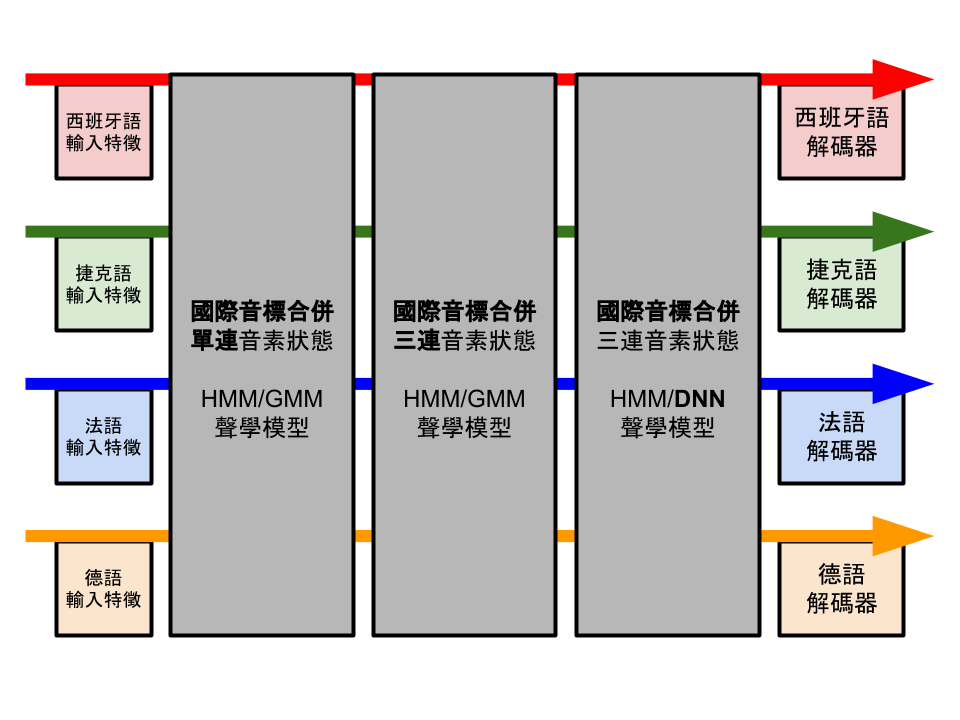
\includegraphics[scale=0.4]{images/chap4_IPA_merged.png}
\caption{基於國際音標合併音素集的西班牙語、捷克語、法語、德語多語音辨識系統}
\label{fig:chap4_IPA_merged}
\end{figure}

圖\ref{fig:chap4_IPA_merged}中,四個語言的資料混合起來,從底層重新開始訓練單連音素HMM/GMM聲學模型、三連音素HMM/GMM聲學模型、三連音素深層類神經網路聲學模型。評估時,四個語言仍然會與相應的辭典以及語言模型結合,形成特定語言的解碼器,產生辨識結果。

\subsection{實驗結果與分析}

\begin{table}[htbp]
%\resizebox{\columnwidth}{!}{
\centering
\begin{tabular}{|c>{\columncolor{red!20}}c>{\columncolor{green!20}}c>{\columncolor{blue!20}}c>{\columncolor{yellow!20}}c>{\columncolor{gray}}cc|}
\hline
 方法 & 西語 & 捷克 & 法語 & 德語 & AWERR & 參數數量 \\
\hline
  單語言基準實驗 & 8.74\% & 18.16\% & 17.43\% & 15.85\% & 100\% & 75.6M \\
\hline
  6073個狀態 & 10.03\% & 18.89\% & 18.78\% & 17.27\% & 108.8\% & 26.3M \\
\hline
  7633個狀態 & 9.53\% & 19.13\% & 18.60\% & 17.08\%  & 107.2\% & 29.5M\\
\hline
  8010個狀態 & 9.51\% & 18.80\% & 18.56\% & 16.78\%  & 106.2\% & 30.3M\\
\hline
\end{tabular}
\caption{基於國際音標合併的多語言辨識系統詞錯誤率,與單語言基準實驗比較。表中的深層類神經網路模型都是4層寬度2048神經元,使用S型函數且未使用丟棄演算法。合併後的模型參數數量減少許多,是因為四個語言間共用了大量的深層類神經網路參數。}
\label{table:chap4_IPA_merged}
\end{table}

表\ref{table:chap4_IPA_merged}為辨識結果評估,無論是哪一個語言,詞錯誤率都比單語言的基準實驗高,因此AWERR是大於100\%的數字。基於國際音標合併多語言的音素集,顯然沒有幫助個別語言的詞錯誤率下降,各個語言使用自己的單語言辨識系統結果都較好。

分析實驗結果,推斷可能的原因為:
\begin{itemize}
 \itemsep -2pt
  \item 將各個語言的音素集合併形成全域音素集後,總計會有80個音素,使得訓練考量前後文相依的三連音素聲學模型時,模型複雜度三次方上升,所需的訓練資料量嚴重不足,使得聲學模型無法訓練完全。
  \item 有些音素獨立於其他音素之外,不會與其他語言共用的特定語言音素,合併後情況依然。然而在訓練深層類神經網路時,該資料量相較於整體資料量的比例會因此下降,造成事前機率過低,不容易被辨識出來。
  \item 即便被分類在同樣的國際音標符號,不同語言的音素仍然會有差異。被標成同樣IPA符號的音素,有大部分於人耳聽起來根本不同,合併其實沒有互相傳授跨語言知識的意義。
\end{itemize}

然而,考量到深層類神經網路模型的參數數量時,會發現這個方法具有有損壓縮(Lossy compression)的效果。基於國際音標合併音素的多語言語音辨識系統,會在不同語言中共享深層類神經網路模型,比起單語言語音辨識系統,能夠節省59\% 到 65\%的模型參數數量,但會增加6.2\% 到 8.8\%的AWERR。隨著參數數量增加,壓縮效果減少,辨識結果相對變好,有折衷(trade-off)空間。

\section{基於資料混淆矩陣的音素狀態合併}
上節基於國際音標合併音素,是根據人耳對於發音單位的鑑別力,來進行合併。然在機器層面上,音素層級的發音單位太過粗糙。本論文著眼於這個點,探討一個更細緻的合併方法,也就是本節資料導向(Data-driven)以混淆矩陣(Confusion Matrix)的三連音素狀態合併。


\subsection{混淆矩陣}
三連音素狀態,是在聲學模型訓練過程中分割單連音素狀態而成的更細緻發音單位,本身就是來自於資料特性所形成的,因此缺少了語言學家的標定,無法藉由知識標記不同狀態的相似性。因此,本論文借助資料導向(Data-driven)的方式,建立混淆矩陣(Confusion Matrix, CM)來找出相近的三連音素狀態進行合併。

\begin{figure}[!h]
\centering
\subfloat[][對稱性] {
    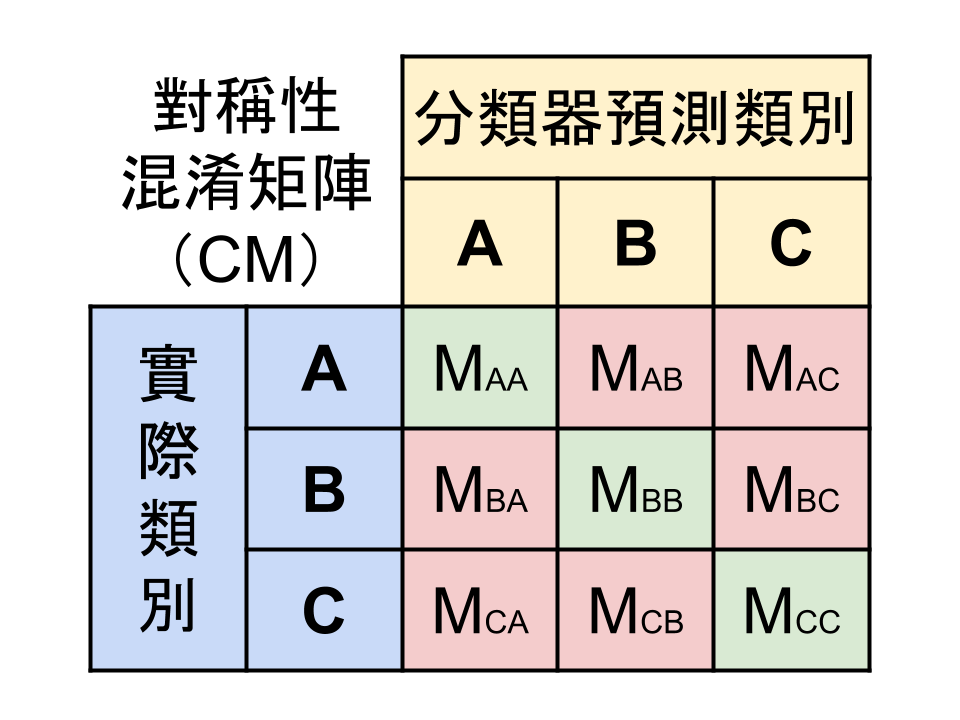
\includegraphics[scale=0.18]{images/chap4_CM.png}
    \label{fig:chap4_CM}
}
\subfloat[][非對稱性] {
    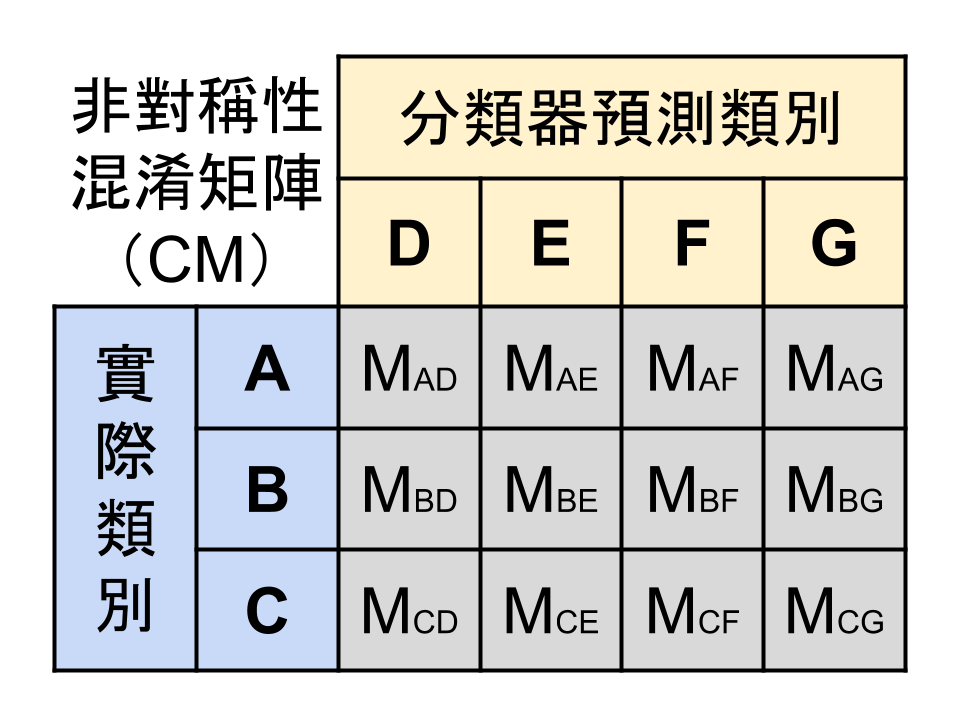
\includegraphics[scale=0.18]{images/chap4_CM_asymm.png}
    \label{fig:chap4_CM_asymm}
}
\caption{典型的混淆矩陣示意圖}
\end{figure}

混淆矩陣(Confusion Matrix),是衡量分類器測試結果時,輔助呈現的一張矩陣式表格。如圖\ref{fig:chap4_CM}中,每一列是實際的類別,而每一行則是預測的類別。矩陣的元素代表的是屬於該實際類別的測試實例中,有多少個被分類為相應的預測實例。藉由表格,就可以算出每個類別的分類精確度(Precision),召回率(Recall)還有準確率(Accuracy)以及F分數(F-score),如公式(\ref{eq:chap4_precision}) 、(\ref{eq:chap4_recall})、(\ref{eq:chap4_fscore})、(\ref{eq:chap4_accuracy})。
\begin{equation}\label{eq:chap4_precision}
Precision(i) = \frac{M_{ii}}{\sum_{j \in \{ A,B,C\}} M_{ji} } 
\end{equation}
\begin{equation}\label{eq:chap4_recall}
Recall(i) = \frac{M_{ii}}{\sum_{j \in \{ A,B,C\}} M_{ij} } 
\end{equation}
\begin{equation}\label{eq:chap4_fscore}
FScore(i) = \frac{2 \times Recall(i) \times Precision(i) }{ Recall(i) + Precision(i)} 
\end{equation}
\begin{equation}\label{eq:chap4_accuracy}
Accuracy = \frac{\sum_{i \in \{ A,B,C\}}M_{ii} }{ \sum_{(i,j) \in \{A,B,C\}^2} M_{ij} }
\end{equation}

對角線的值越高,表示分類器分類在正確的類別的機率越高,則分類器的表現越好。精確度越高,則表示分類器分類結果是對的比例越高;召回率越高,則表示分類器能夠找出正確類別的比例越高。這兩者有著互相折衷的關係,因此可以考量準確度或是F分數來整體評估分類器的結果。

混淆矩陣中,不在對角線的值是該實際類別被分類為該預測類別的數量。數量越多,該實際類別越容易被分類為該預測類別,代表這兩個類別一定有某種程度的相似性,容易造成混淆,混淆矩陣因而有其名。在評估分類器時,混淆矩陣是對稱的(Symmetric),往往需要整體的數據來評估分類器結果。利用混淆矩陣代表相似度、混淆度的特性,當實際類別以及分類類別是不同的集合時,亦可以產生非對稱的混淆矩陣,如圖\ref{fig:chap4_CM_asymm}。

值得一提的是,混淆矩陣是否具有對稱性,根據的是輸入實例的實際類別集是否與分類器預測類別集一致,不是數值矩陣本身的對稱性。如圖\ref{fig:chap4_CM}中,$M_{BA} \neq M_{AB}$,即便他是對稱矩陣。

\begin{figure}[!h]
\centering
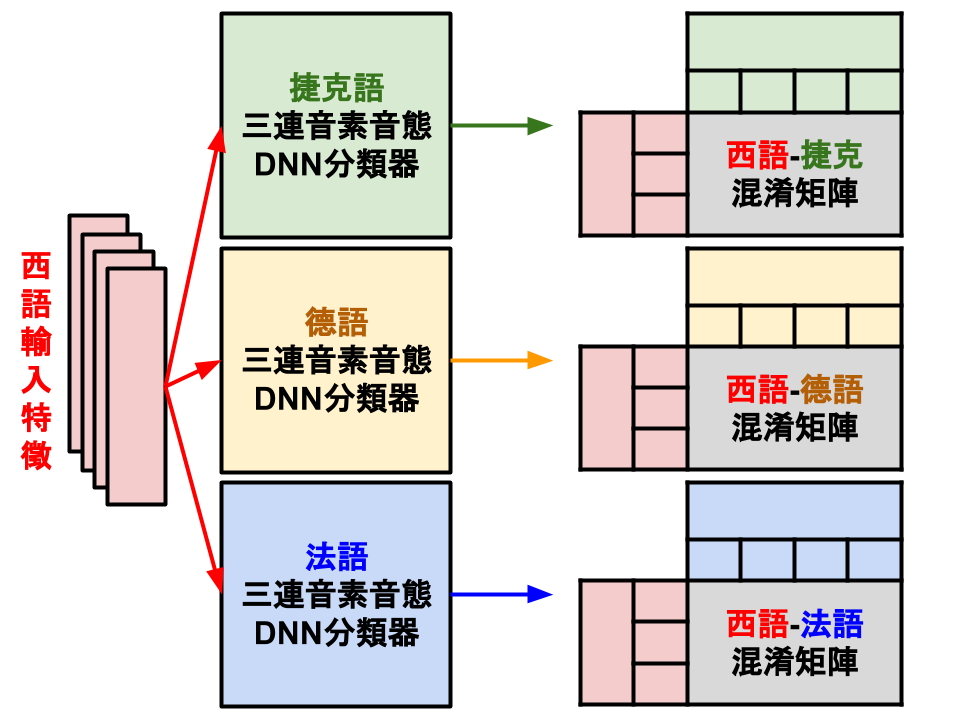
\includegraphics[scale=0.4]{images/chap4_cross_decode.png}
\caption{針對西班牙語言的輸入特徵向量,分別以單語言類神經網路分類器進行捷克語、德語以及法語的交叉解碼(Cross Decode),以計算非對稱混淆矩陣。}
\label{fig:chap4_cross_decode}
\end{figure}

在語音辨識系統中,特定語言語料所訓練的深層類神經網路模型用於給定輸入另一種語言的特徵向量,分類前者的三連音素狀態,如圖\ref{fig:chap4_cross_decode}。如果對西班牙語的輸入特徵向量使用訓練於德語的深層類神經網路進行分類時,即可以得到實際類別為西班牙語三連音素狀態集、預測類別為德語三連音素狀態集的混淆矩陣。依此推類,總計可以產生12組非對稱的混淆矩陣,如公式(\ref{eq:chap4_CM_hard})。
\begin{equation} \label{eq:chap4_CM_hard}
M( s^{(l1)} , s^{(l2)} ) = \sum_{ \bold{x} \in D(s^{l1}) } \mathbbm{1} \{ s^{(l2)} = \arg\max_{i} y_{i}^{(l2)}(\bold{x}) \}
\end{equation}
其中$s^{(l1)}$、$s^{(l2)}$分別是來自語言l1和l2的三連音素狀態,$D(s^{l1})$是語言l1中實際類別為$s^{(l1)}$的輸入訓練特徵向量集,$y_{i}^{(l2)}(\bold{x})$是語言l2的深層類神經網路分類器,在輸入特徵向量$\bold{x}$後,最後一層軟性最大化輸出層的第i維。$\mathbbm{1}\{ \}$ 為指示函數(Indicator Function),當輸入邏輯為真的時候,函數輸出為1,反之則為0。

以深層類神經網路模型進行跨語言分類時,分類器並沒有正確答案,因為本來就屬於不同語言的範疇。但某一項分類的機率越高,代表的是兩個三連音素狀態的近似程度越高。公式(\ref{eq:chap4_CM_hard})使用的是如傳統混淆矩陣的硬式預測(Hard Predicion),但為了得到更豐富的混淆度,可以使用如公式\ref{eq:chap4_CM_soft}的軟式預測(Soft Prediction),把模型分類的機率直接納入考量,而不只是考量最大值,納入較多資訊。
\begin{equation} \label{eq:chap4_CM_soft}
M( s^{(l1)} , s^{(l2)} ) = \sum_{ \bold{x} \in D(s^{l1}) } y_{i}^{(l2)}(\bold{x}) 
\end{equation}

有了軟式混淆矩陣,再除以實際音素的數量,即可以獲得非對稱的相似度(Asymmetric Similarity),如式\ref{eq:chap4_asym_sim}。
\begin{equation} \label{eq:chap4_asym_sim}
ASIM( s^{(l1)} , s^{(l2)} ) =  \frac{ M( s^{(l1)} , s^{(l2)}) } { count( s^{(l1)} )}
\end{equation}

每對不同語言的三連音素狀態,會有兩個混淆矩陣算出來的非對稱相似度,如公式\ref{eq:chap4_sym_sim}平均後,即為這兩個三連音素狀態的對稱相似度(Symmertric Similarity)。
\begin{equation} \label{eq:chap4_sym_sim}
SIM( s^{(l1)} , s^{(l2)} ) =  \frac{ ASIM( s^{(l1)} , s^{(l2)})  + ASIM( s^{(l2)} , s^{(l1)})} {2 }
\end{equation}
\subsection{階層式累積分群合併}

階層式累積分群(Hierarchical Agglomerative Clustering, HAC)是一個非監督式分群方法,給定各個訓練實例在空間中的距離,由下而上合併實例,最後停在足夠概括的分群設定下。演算法設定與步驟如下:

\begin{itemize}
 \itemsep -2pt
 \item 計算語言間所有三連音素狀態之間的對稱相似度,如公式\ref{eq:chap4_sym_sim}。
 \item 找出相似度最高的一對三連音素狀態$( s^{(l1)} , s^{(l2)}  )$。
 \item 如果這組三連音素狀態已經合併過,或是合併後會導致有同語言的三連音素狀態被合併在一起,則不合併這組。
 \item 持續找出最大的相似度並且合併三連音素狀態,直到合併到指定的三連音素狀態數量。
\end{itemize}

如圖\ref{fig:chap4_hac},同一語言的三連音素狀態,在訓練聲學模型時就已經強制分開,因此在階層式分群合併跨語言音素時,不會再進行合併。

\begin{figure}[!h]
\centering
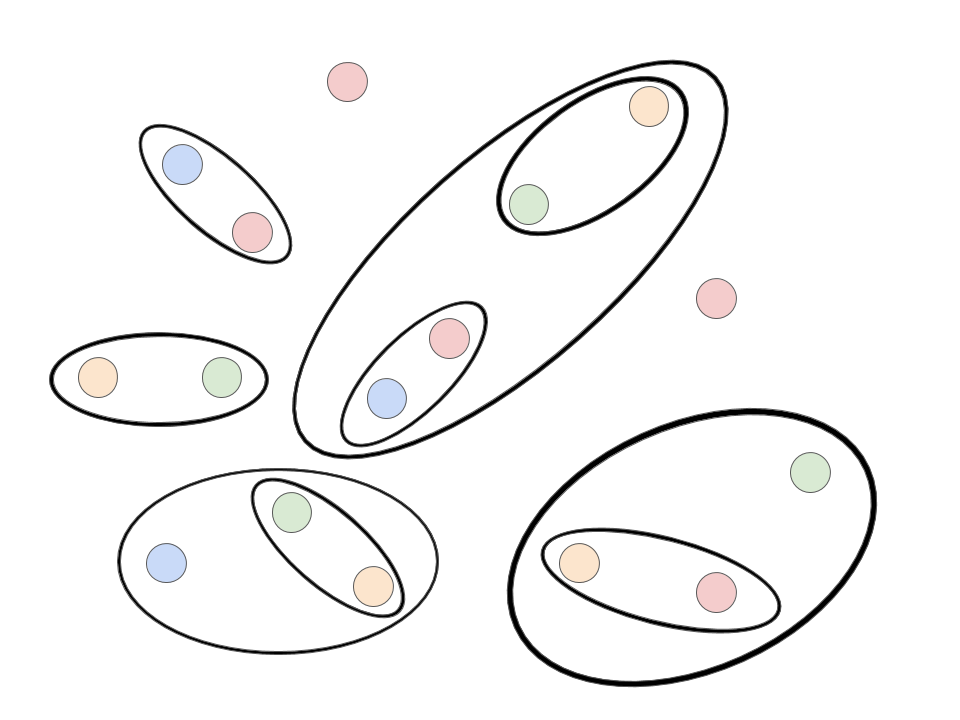
\includegraphics[scale=0.4]{images/chap4_hac.png}
\caption{階層式累積分群合併示意圖。圖中不同顏色的原點代表四個語言的三連音素狀態分佈在空間中,黑色圈圈為合併的結果。合併過程會優先將鄰近的音素狀態合併起來,但不會將同一個語言的音素狀態合併,因此每一群最多只會有四個原點。}
\label{fig:chap4_hac}
\end{figure}


\begin{table}[!h]
%\resizebox{\columnwidth}{!}{
\centering
\begin{tabular}{|cccc|}
\hline
\# & 相似度   & 三連音素狀態    & 三連音素狀態    \\
\hline
2  & 0.691 & 捷克753(s)  & 西語690(s)  \\
\hline
12 & 0.571 & 法語579(S)  & 德語1051(z) \\
\hline
16 & 0.558 & 法語580(AE) & 德語1048(x) \\
\hline
19 & 0.541 & 法語1407(a) & 西語187(a) \\
\hline
\end{tabular}
\caption{基於混淆矩陣合併三連音素狀態,第一行為合併的優先序。三連音素狀態除了編號之外,括號內顯示其中間音素。}
\label{table:chap4_CM_merge_examples}
\end{table}
表\ref{table:chap4_CM_merge_examples}為合併的實例。為了語音辨識系統穩健性,通常會在發音單位中加上沉默(Silence, sil)當作一種音素,儘管他意味著不發音。大部分的合併都是沉默狀態的合併,不列在表上。從表格看來,基於混淆矩陣合併三連音素狀態,其中間的音素在語言學上亦是接近的單位,如法語的S與德語的z。但實際上合併的則是法語編號579以及德語編號1051的三連音素狀態,比音素細緻且人耳無法辨識。

從表\ref{table:chap4_CM_merge_examples}中可以看到如順序16,法語的580以及德語的1048,兩個三連音素狀態的中間音素並不相似,在語言學無法解釋其資料的相似性。

\subsection{合併三連音素狀態的多語言語音辨識系統}

基於混淆矩陣合併好三連音素狀態,整體的系統架構如圖\ref{fig:chap4_CM_framework}。在訓練單語言語音辨識系統時,每個語言會先訓練單連音素狀態與三連音素狀態的聲學模型。但在訓練深層類神經網路聲學模型時,會把四個語言的三連音素狀態合併起來訓練,形成多語言語音辨識系統。
\begin{figure}[!h]
\centering
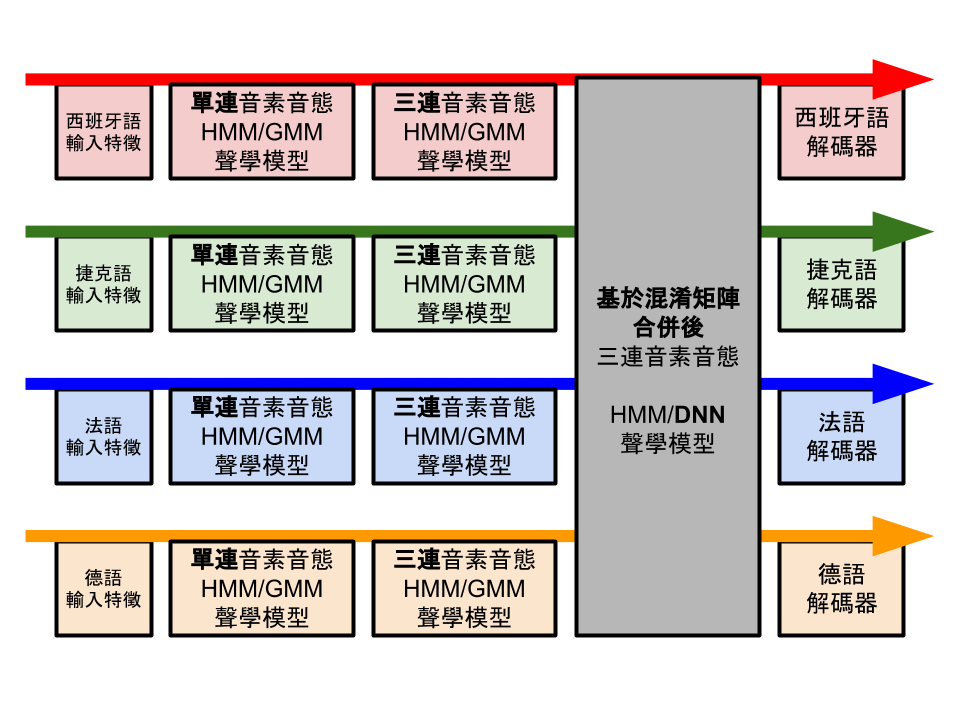
\includegraphics[scale=0.4]{images/chap4_CM_merged.png}
\caption{基於混淆矩陣合併三連音素狀態,多語言語音辨識系統訓練架構圖。其中每個語言訓練的前兩個階段,與單語言語音辨識系統相同。}
\label{fig:chap4_CM_framework}
\end{figure}

經過階層式合併,原本屬於各自語言的三連音素狀態,會與相近的其他語言三連音素狀態合併,再由深層類神經網路模型去預測合併後的類別,形成如圖\ref{fig:chap4_CM_merged_unit}的分類器架構。深層類神經網路輸出的最後一層邏輯子,會以跨語言三連音素狀態的方式訓練,但會在解碼時對應回該特定語言的三連音素狀態,形成包含多語言知識的單語言語音辨識解碼器。
\begin{figure}[!h]
\centering
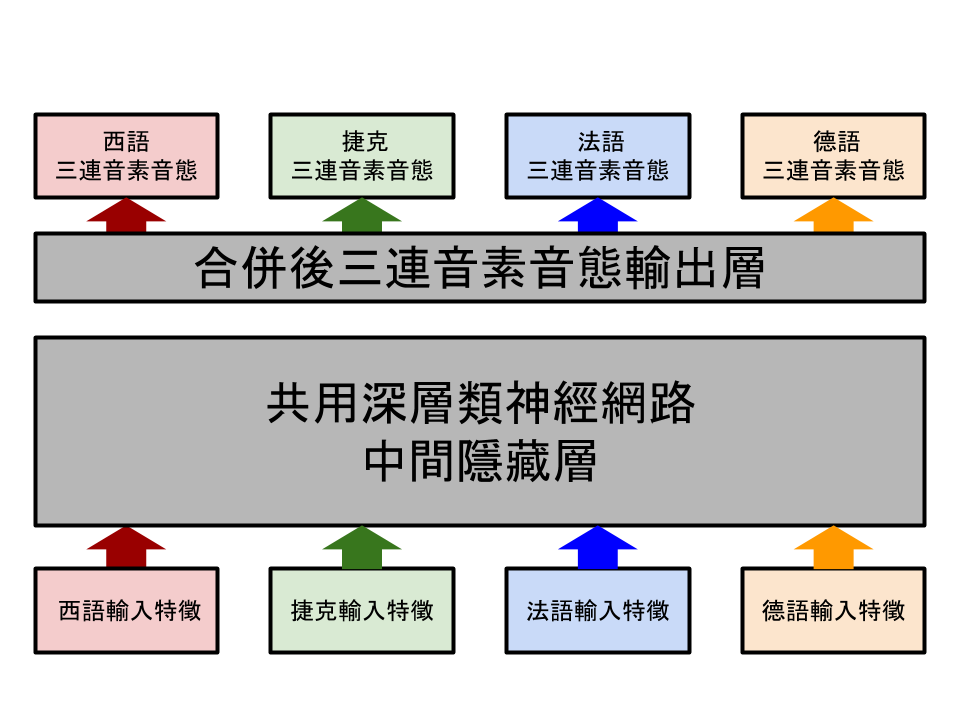
\includegraphics[scale=0.4]{images/chap4_CM_merged_unit}
\caption{基於混淆矩陣合併三連音素狀態,多語言語音辨識系統的深層類神經網路訓練示意圖。}
\label{fig:chap4_CM_merged_unit}
\end{figure}

\subsection{加上國際音標限制}
基於國際音標合併發音單位的方式,是純粹基於語言學上的知識,但只能提供較粗的音素層級的合併;基於混淆矩陣合併三連音素狀態的方式,是純粹考量資料分佈的混淆程度,誤差會干擾其中的結果。圖\ref{fig:chap4_CM_IPA}為法語與西語間的混淆矩陣。

\begin{figure}[!h]
\centering
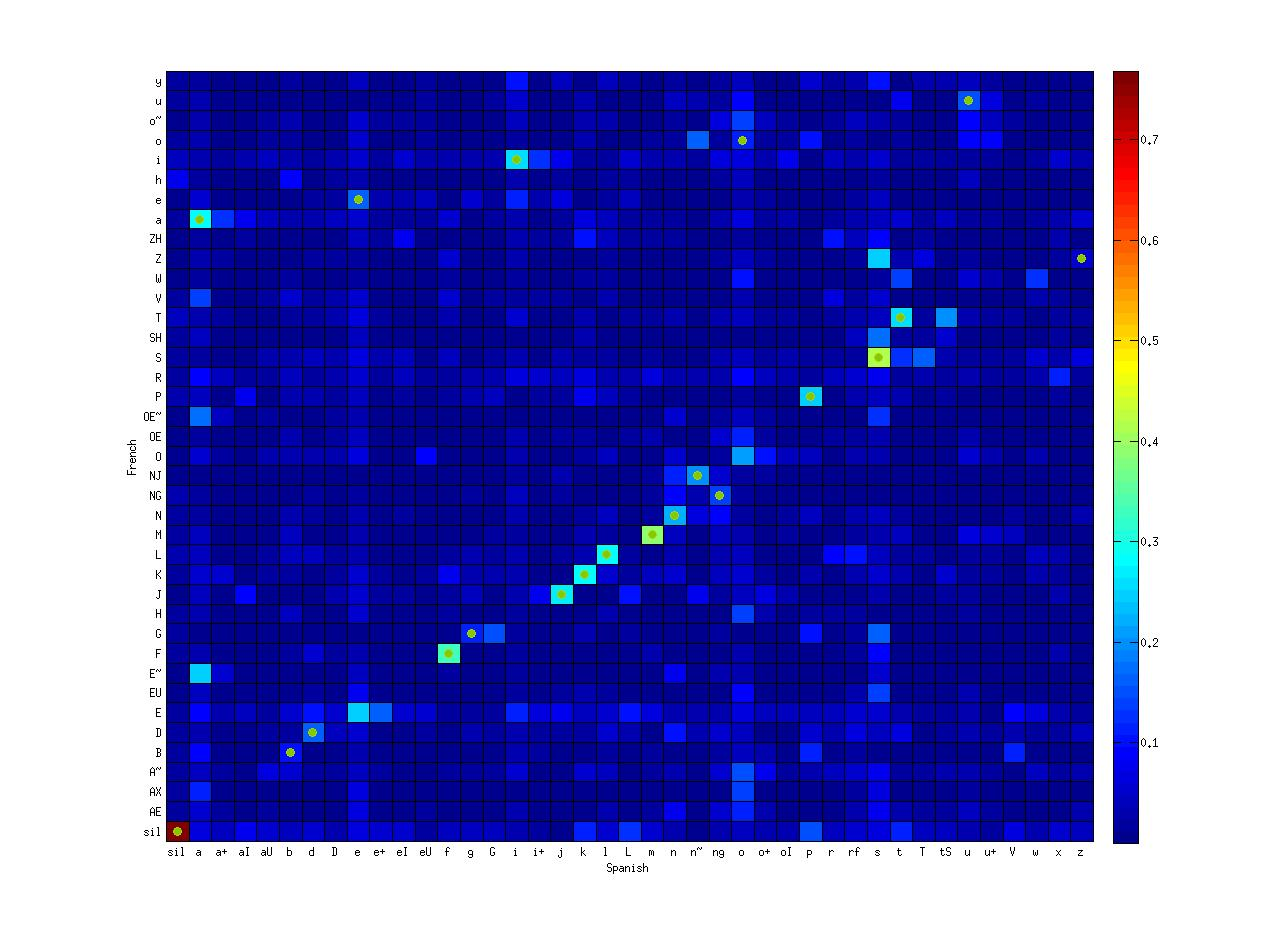
\includegraphics[scale=0.3]{images/chap4_CM_IPA}
\caption{法語對於西語的非對稱相似度混淆矩陣,合併成音素層級。橫軸是法語的音素,縱軸是西語的音素。矩陣元素的顏色代表相似度的值,越深藍越低,越黃紅越高。綠色圓點代表國際音標屬於同一個符號的組合。左下角的沉默音素顯然擁有極高的相似度。}
\label{fig:chap4_CM_IPA}
\end{figure}

為了方便理解發音單位之間的關聯,圖\ref{fig:chap4_CM_IPA}將三連音素狀態根據中央音素合併為較粗的音素單位呈現,綠色的圓點代表兩個音素在國際音標中被標定為相同的符號。

圖\ref{fig:chap4_CM_IPA}中大部份的顏色偏藍色系,代表的是混淆度不高,即大部分的音素彼此不容易混淆;然而顏色偏亮偏黃的,即為資料混淆度較高的音素。由圖中可知,混淆程度高的部份大致和國際音標的合併趨勢相符,但混淆矩陣仍明顯顯示在有些音素對應關係中呈現高混淆度。

如果純粹基於混淆矩陣合併三連音素狀態,雖然能夠合併比較細緻的發音單位,卻缺少了語言學的限制,有可能將不合理的發音單位合併起來。

為了避免誤差影響合併結果,在合併三連音素狀態時,可以在階層式分群時加入語言知識的限制,亦即當兩個三連音素狀態的中央音素不屬於同一個國際音標符號,兩狀態就不能合併。

\subsection{實驗結果與分析}

\begin{table}[htbp]
%\resizebox{\columnwidth}{!}{
\centering
\begin{tabular}{|c>{\columncolor{red!20}}c>{\columncolor{green!20}}c>{\columncolor{blue!20}}c>{\columncolor{yellow!20}}c>{\columncolor{gray}}cc|}
\hline
 方法 & 西語 & 捷克 & 法語 & 德語 & AWERR & 參數數量 \\
\hline
  (1) 單語言基準實驗 & 8.74\% & 18.16\% & 17.43\% & 15.85\% & 100\% & 75.6M \\
\hline
  (2) 國際音標(6073) & 10.03\% & 18.89\% & 18.78\% & 17.27\% & 108.8\% & 26.3M \\
\hline
  (3) 混淆矩陣(6073) & 8.78\% & 18.01\% & 17.54\% & 14.75\% & 98.28\% & 26.3M \\
  (4) +國際音標限制 & 8.83\% & 18.09\% & 17.66\% & 16.06\% & 100.82\% & 26.3M \\
\hline
  (5) 國際音標(7633) & 9.53\% & 19.13\% & 18.60\% & 17.08\%  & 107.2\% & 29.5M\\
\hline
  (6) 混淆矩陣(7633) & 8.67\% & 17.89\% & 17.50\% & 15.16\%  & 98.42\% & 29.5M\\
\hline
  (7) 國際音標(8010) & 9.51\% & 18.80\% & 18.56\% & 16.78\%  & 106.2\% & 30.3M\\
\hline
  (8) 混淆矩陣(8010) & 8.87\% & 17.82\% & 17.68\% & 15.32\%  & 99.4\% & 30.3M\\
\hline
\end{tabular}
\caption{基於混淆矩陣合併三連音素狀態之多語言語音辨識系統,與基準實驗還有國際音標合併的實驗比較。括號內是合併後的三連音素狀態數量。表中的聲學模型都是使用S型函數深度4層,寬度為2048神經元的深層類神經網路。(1)為表\ref{table:chap3_dropout}中使用S型函數的基準實驗,為計算AWERR的基準。(2)(5)(7)為表\ref{table:chap4_IPA_merged}中合併國際音標實驗中,不同音素狀態設定的結果。(3)(6)(8)為本節使用混淆矩陣合併音素狀態後的結果,刻意設定與國際音素合併的設定相同,以方便比較。(4)為實驗(3)的設定下,額外添加國際音標限制。}
\label{table:chap4_CM_merged}
\end{table}

表\ref{table:chap4_CM_merged}為實驗結果,為了控制在相同的參數數量方便比較結果,在階層式分群時,設定合併的三連音素狀態的數量與表\ref{table:chap4_IPA_merged}相同。

表中可以看到,基於混淆矩陣合併三連音素狀態(3)(6)(8),不僅整體的表現都比單語言語音辨識系統(1)好,參數數量也跟國際音標合併的深層類神經網路(2)(5)(7)一樣。這個方法成功借助其他語言的資訊,輔助本身語言的學習,藉由合併細緻的三連音素狀態,提升資料量。

此外,表\ref{table:chap4_IPA_merged}中可以看到,在基於混淆矩陣合併三連音素狀態時,如果加上國際音標的限制如實驗(4),都沒有使得結果變得更好。這表示語言知識的限制反而干擾了資料混淆矩陣所呈現的相似度,使得階層式分群時較難將相近的三連音素狀態合併起來,共享深層類神經網路訓練。

由這些結果可知,基於混淆矩陣合併三連音素狀態的多語言語音辨識系統,可以成功降低詞錯誤率以及參數數量,利用模型共享增加資料量,幫助深層類神經網路聲學模型學習。相比於基於國際音標合併音素的多語言語音辨識系統,成功的原因在於找出更細緻的發音單位合併方式。

\section{基於模型共享的中間層合併}
\subsection{深層神經網路中間層合併}
鑒於合併三連音素狀態的成功,更深入的研究在於如何找到更細緻的合併方式。以深層類神經網路模型作為三連音素狀態分類器的過程中,中間的隱藏層在訓練過程,由淺至深逐漸學習到時頻資訊以及語音資訊,在最後一層的時候,輔助三連音素狀態的分類。

因此,如果將合併層級,從分類器最後輸出層的三連音素狀態,往前推移到更細緻的深層類神經網路中間層,而讓最後一層分類器能夠根據不同語言有不同的輸出層。

藉由共享深層類神經網路模型的中間層,可以讓模型學習到跨語言的聲音資訊,形成跨語言特徵萃取器,與各語言的專屬三連狀態分類器,同時訓練,如圖\ref{fig:chap4_dnn_sharing}。
\begin{figure}[!h]
\centering
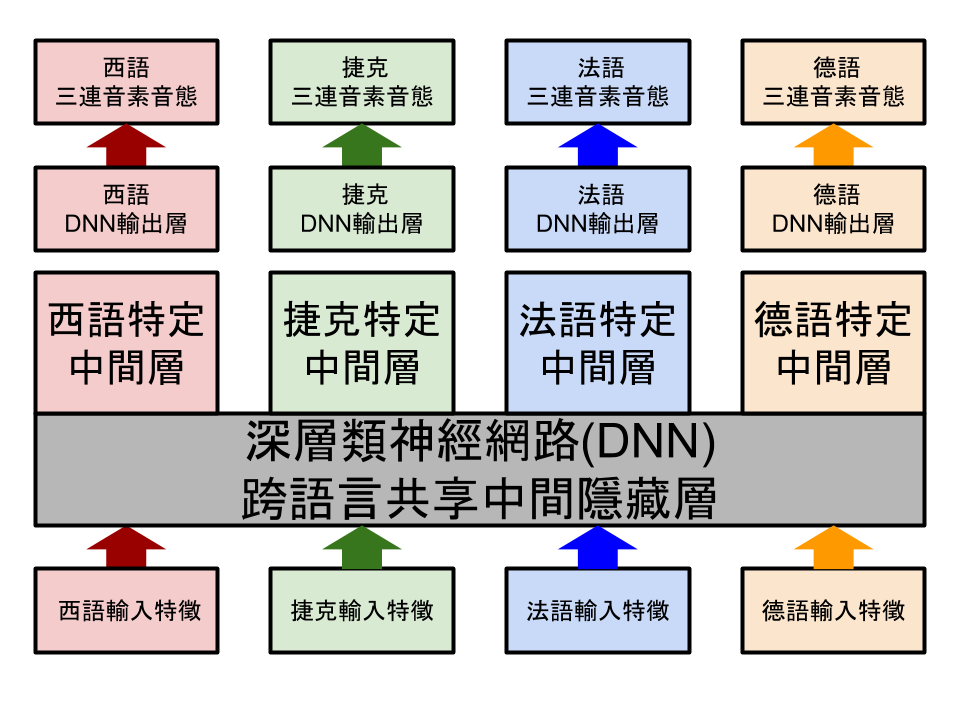
\includegraphics[scale=0.4]{images/chap4_dnn_sharing.png}
\caption{基於模型共享的中間層合併,多語言語音辨識系統中的深層類神經網路模型訓練示意圖。模型的輸出層並沒有合併發音單位,只合併模型前端中間層的參數。}
\label{fig:chap4_dnn_sharing}
\end{figure}

但深層類神經網路模型的參數非常多,一層一層疊加,中間層到底學到什麼樣的資訊,都是在反向傳播過程中自動學習而成,無法分析得知,有不少學者亦致力於其中研究\cite{nagamine2015exploring}。因此,在共享時,哪些中間層該共享學習,是核心的關鍵。

深層類神經網路模型中,越靠近輸入端的中間層,越是能夠學習底層訊號端的知識,其中包含人類語音訊號的頻譜特徵。對於這個底層資訊,有兩種可能的假設:
\begin{itemize}
 \itemsep -2pt
 \item 如果這個底層資訊與語言特色高度相關,共用參數會讓模型受其他語言的資料影響與混淆.訓練效果不彰。分別使用不同的參數,才有足夠的模型能耐學習到語言專屬特色,如圖\ref{fig:chap4_dnn_input_nonsharing}。
 \item 如果這個底層資訊橫跨語言,包含的是語言間共同的頻譜資訊,共用參數會讓模型獲得更加概括化的能力,不僅能降噪,亦能成為很好的特徵萃取器,如圖\ref{fig:chap4_dnn_input_sharing}。
\end{itemize}

\begin{figure}[!h]
\centering
\subfloat[][輸入層不共享] {
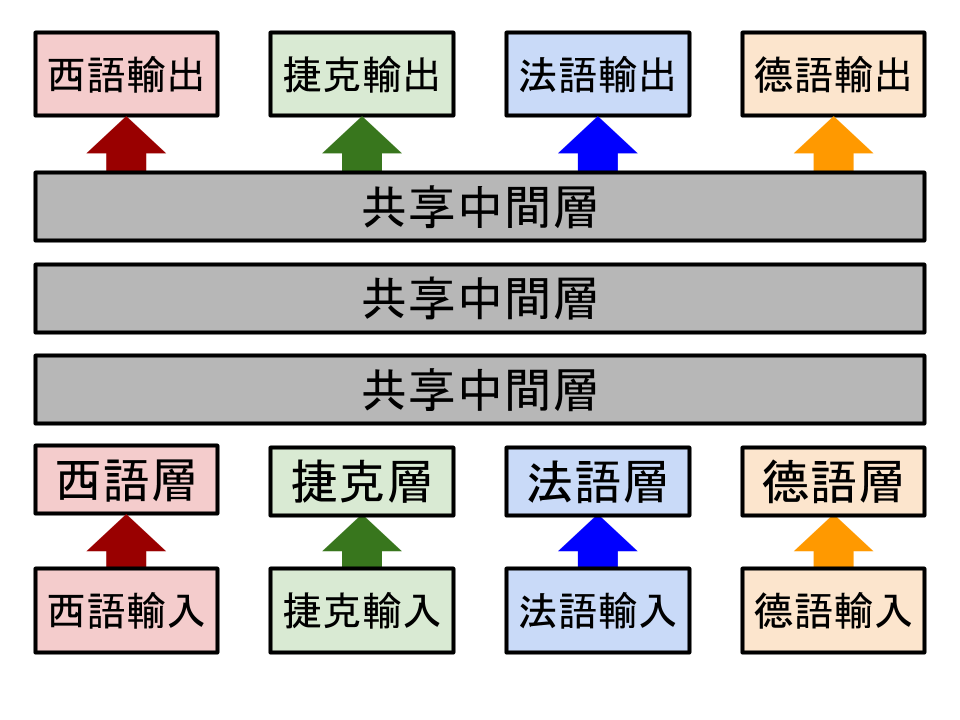
\includegraphics[scale=0.18]{images/chap4_dnn_input_nonsharing.png}
\label{fig:chap4_dnn_input_nonsharing}
}
\subfloat[][全部共享] {
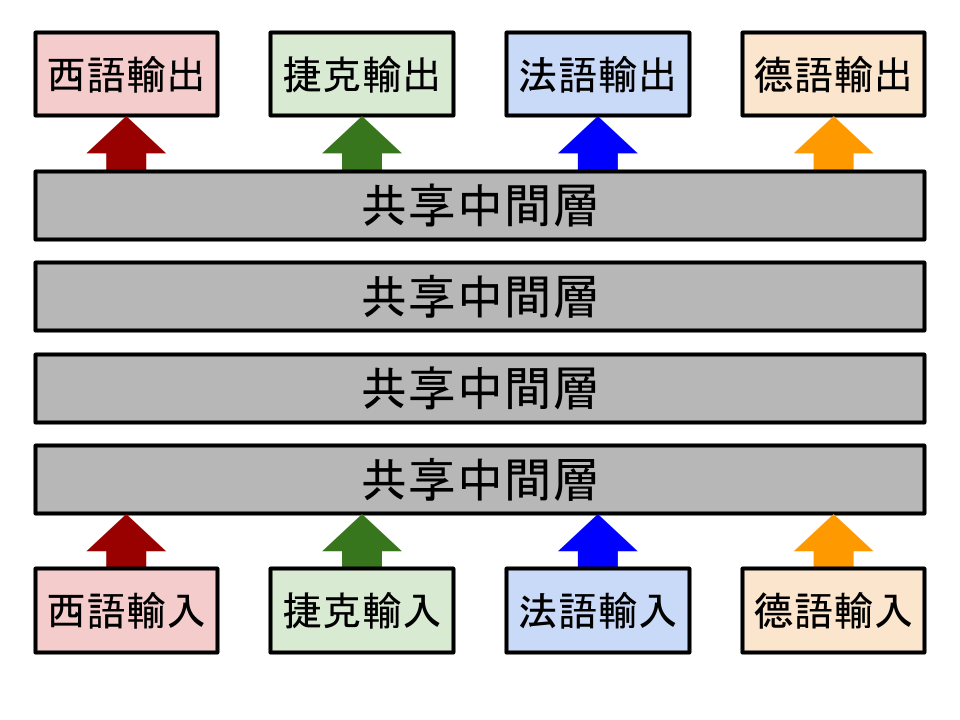
\includegraphics[scale=0.18]{images/chap4_dnn_input_sharing.png}
\label{fig:chap4_dnn_input_sharing}
}
\caption{基於模型共享的中間層合併,兩種可能共享設定。}
\end{figure}

模型中越靠近輸出端的中間層,包含的是高階的語言專屬知識,以提供分類器區分三連音素狀態。
\subsection{實驗結果與比較}

\begin{table}[htbp]
%\resizebox{\columnwidth}{!}{
\centering
\caption{基於模型共享的中間層合併,多語言語音辨識系統的實驗結果。表中的聲學模型都是使用S型函數深度4層,寬度為2048神經元的深層類神經網路。}
\label{table:chap4_dnn_sharing_baseline}
\begin{tabular}{|c>{\columncolor{red!20}}c>{\columncolor{green!20}}c>{\columncolor{blue!20}}c>{\columncolor{yellow!20}}c>{\columncolor{gray}}cc|}
\hline
 方法 & 西語 & 捷克 & 法語 & 德語 & AWERR & 參數數量 \\
\hline
  單語言基準實驗 & 8.74\% & 18.16\% & 17.43\% & 15.85\% & 100\% & 75.6M \\
\hline
  輸入層不共享 & 8.90\% & 18.09\% & 17.69\% & 15.32\% & 99.88\% & 40.2M \\
\hline
  中間層全部共享 & 8.50\% & 17.73\% & 18.05\% & 14.28\% & 97.02\% & 36.4M \\
%\hline
%  輸出層前兩層不共享 & 8.72\% & 18.16\% & 18.61\% & 14.75\%  & 99.78\% & 49.0M\\
\hline
\end{tabular}
\end{table}

表\ref{table:chap4_dnn_sharing_baseline}為模型共享的基準實驗,與單語言語音辨識系統的結果比較。輸入層不共享的結果比全部共享來得較差,表示靠近輸入層的中間層應包含跨語言的頻譜知識,進行跨語言訓練能夠增加資料量幫助訓練。

%原本預期靠近輸出層的中間層富含較多的語言特定知識,但從表\ref{table:chap4_dnn_sharing_baseline}中的結果顯示,輸出層前兩層不共享的結果比全部中間層共享的結果差,推測是深度不足,4層的資訊如果共用仍然能學到更多的東西。

\begin{table}[htbp]
%\resizebox{\columnwidth}{!}{
\centering
\begin{tabular}{|c>{\columncolor{red!20}}c>{\columncolor{green!20}}c>{\columncolor{blue!20}}c>{\columncolor{yellow!20}}c>{\columncolor{gray}}cc|}
\hline
 方法 & 西語 & 捷克 & 法語 & 德語 & AWERR & 參數數量 \\
\hline
  (1)單語言4層基準實驗 & 8.74\% & 18.16\% & 17.43\% & 15.85\% & 100\% & 75.6M \\
  (2)+線性整流與丟棄0.1 & 8.58\% & 17.61\% & 17.15\% & 15.40\% & 97.67\% & 75.6M \\
  (3)+增加至7層中間層 & 8.41\% & 17.03\% & 16.80\% & 14.50\% & 94.45\% & 128.3M \\
\hline
  (4)4層共享中間層 & 8.50\% & 17.73\% & 18.05\% & 14.28\% & 97.02\% & 36.4M \\
  (5)+線性整流與丟棄0.1 & 8.29\% & 17.05\% & 16.93\% & 14.15\% & 93.74\% & 36.4M \\
  (6)+增加至7層共享中間層 & 8.10\% & 16.75\% & 16.65\% & 12.95\% & 90.38\% & 49.9M \\
%\hline
%  前4層共享+後3層不共享 & 7.96\% & 16.56\% & 16.42\% & 13.57\%  & 90.47\% & 86.8M\\
\hline
\end{tabular}
\caption{基於模型共享的中間層合併,多語言語音辨識系統的實驗結果。表中的聲學模型都是使用寬度為2048神經元的深層類神經網路。}
\label{table:chap4_dnn_sharing}
\end{table}
表\ref{table:chap4_dnn_sharing}將單語言基準實驗時的丟棄演算法加入比較,並且增加深度,結果與表\ref{table:chap3_dropout}和表\ref{table:chap3_depth}一致,使用丟棄演算法和增加深度都能使結果變好,但仍需要注意到參數數量的提升。
\section{本章實驗比較與綜合分析}
\begin{table}[]
%\resizebox{\columnwidth}{!}{
\centering
\begin{tabular}{|c|c|c|c|c|}
\hline
\multirow{2}{*}{方式} & \multirow{2}{*}{AWERR}    & 是否合併& 是否合併             & 是否合併 \\
     & & DNN  & 三連音素狀態 &  聲學模型轉移模型 \\
\hline
單語言基礎實驗  & 100\% &  &  &   \\
\hline
(1) 基於國際音標 & \multirow{2}{*}{106.2\% } & \multirow{2}{*}{ 是 } & \multirow{2}{*}{是}  & \multirow{2}{*}{是}  \\
合併音素& & & & \\
\hline
(2) 基於混淆矩陣 & \multirow{2}{*}{ 98.28\%} & \multirow{2}{*}{ 是 } & \multirow{2}{*}{是}  &  \\
合併三連音素狀態& & & & \\
\hline
(3) 基於模型共享 & \multirow{2}{*}{97.02\%} &\multirow{2}{*}{ 是 } &  &  \\
合併中間層 & & & & \\
\hline
\end{tabular}
\caption{本章三種合併發音單位的實驗比較,用以訓練多語言語音辨識系統內的深層類神經網絡模型。表中數據都使用S型函數、深度為4層、寬度為2048神經元的模型中,該方法下最好的AWERR結果,與表\ref{table:chap4_IPA_merged} 8010個狀態、表\ref{table:chap4_CM_merged} 6073個狀態以及表\ref{table:chap4_dnn_sharing_baseline} 全部共享一致。}
\label{table:chap4_merging_illustrator}
\end{table}
多語言語音辨識聲學模型中,深度類神經網路佔據著不可或缺的地位,然其訓練過程需要特別多的資料量,如果能從其他語言中借助更多的資料幫助訓練,增強模型潛力。

然所謂的更多資料,充其量也只是更多充滿雜訊的不匹配資料而已,從機器學習的角度上來看,甚至會干擾模型的學習,必須找到可以合併共享的部分,只學習合適且重要的資訊來達到目標。

本章從音素合併模型,開始逐步磨細成三連音素狀態合併,最後停在深層類神經網路模型的中間層合併,整體的脈絡如表\ref{table:chap4_merging_illustrator},由粗糙到細緻的發音單位合併。

即便人耳最多只能鑑別音素,有許多差異是只有機器才能區別出來。這些橫跨語言的知識,與語言特性高度相關。本研究使用的四個語言都是印歐語系,但是屬於不同分支,因此仍然可以從中看到多語言語音辨識系統架構設計上的蹊蹺。

\chapter{知識蒸餾(Knowledge Distillation)}
  \section{簡介}
\section{溫度軟性最大化(Temperature Softmax)}
\section{蒸餾設定與步驟}
\section{多目標蒸餾}
\subsection{多個單語言老師模型}
\subsection{單個多語言老師模型}
\section{蒸餾與模型壓縮}
\section{實驗結果與分析}
\subsection{溫度}
\subsection{老師模型}
\subsection{模型壓縮}
\subsection{綜合比較}    


\chapter{結論與展望}
  \section{本論文主要的研究貢獻}

本論文旨在探討聲學模型中的深度學習架構,並且套用於多語言情境之下,探討如何增加深度學習的資料量,形成跨語言類神經網路。主要的研究貢獻如下:

\begin{itemize}
 \itemsep -2pt
 \item 本論文先回顧基本的單語言語音辨識系統架構,著重在聲學模型中的類神經網路模型,加上現在深度學習中典型的的線性整流活化函數與丟棄演算法,成功從全球音素語料庫的四個語言:西班牙語、捷克語、法語、德語,建立可供比較的單語言語音辨識系統,與全球結果比較。

 \item 提出一個多語言語音辨識系統情境,探討如何產生一種跨語言聲學模型架構,讓四種語言的資料彼此共享訓練,幫助訓練,使得整體需要的資料量變小、模型參數需求也變小。為了評估系統在多語言的表現,提出了平均詞誤率比(AWERR)來衡量整體的辨識結果。

 \item 本論文從聲學模型合併的角度切入,討論基於國際音標合併音素、基於混淆矩陣合併三連音素音態以及基於模型共享合併中間層的方式,由粗糙到細緻層層合併,成功訓練出多語言深層類神經網路,建立比單語言語音辨識系統還要好的跨語言聲學模型。

 \item 多語言語音辨識的訓練過程龐大,與應用層面有所差距,但與知識蒸餾提出的訓練-測試分離概念有所共鳴。本論文探討了單個多語言教師模型的蒸餾,和多個單語言教師模型的蒸餾,將水平共享資訊與垂直蒸餾資訊合併,合併龐大的教師模型知識與廣闊的跨語言共享知識,獲得更好的辨識結果。
\end{itemize}
\section{本論文未來研究方向}

本論文礙於研究之力,有許多可行的想法尚未實現。如以深度學習建立單語言語音辨識系統聲學模型中,已經出現不少使用卷積類神經網路(CNN)或是長短期記憶類神經網路(LSTM)的架構,呈現的數據都相當的好。在訓練深層類神經網路模型的優化演算法上,亦有不少更勝於統計式梯度降低法(SGD)的研究。

本論文使用的基準實驗仍有許多進步的空間,隨著研究蓬勃發展,基準實驗勢必得提升成更經典有效的方法,以探討多語言情境下的各種方式成效。

本論文使研究所使用的四個語言都是印歐語系的。如果要將研究內容探討到更全域的語言特色,勢必得加入更多其他語系的語言討論,甚至是稀少語言的訓練方法。

基於混淆矩陣合併三連音素音態時,以對稱相似度作為合併距離的,並且使用階層式分群法的其中一種進行合併。未來可以使用不同的合併演算法、不同的距離衡量方式,來決定如何合併三連音素音態。

除了基於隱藏式馬可夫模型的聲學模型之外,端至端(End-to-End)系統也逐漸熱門而且效果卓越,其模型中央並沒有所謂的發音單位的概念,探討如何進行多語言模型合併會是個前所未見且有趣的題目。

眼下亦沒有人提出一個對於知識蒸餾概念中的概括化資訊的量化解釋,以及概括化資訊如何幫助類神經網路進行學習。對於概括化資訊中的純理論分析,如與控制調適的關係、與資料揀選的關係,都是值得深入討論的研究部份。


%
% this file is encoded in utf-8
% v2.0 (Apr. 5, 2009)

%%% 參考文獻
\newpage
\phantomsection % for hyperref to register this
\addcontentsline{toc}{chapter}{\nameRef}
\renewcommand{\bibname}{\protect\makebox[5cm][s]{\nameRef}}
%  \makebox{} is fragile; need protect
\bibliographystyle{IEEEbib}  % 使用 IEEE Trans 期刊格式
\bibliography{thesis_bib}


%%% 
%\input{my_appendix.tex}

%%% 自傳
%\newpage
%\chapter*{\protect\makebox[5cm][s]{\nameVita}} % \makebox{} is fragile; need protect
%\phantomsection % for hyperref to register this
%\addcontentsline{toc}{chapter}{\nameVita}
%\input{my_vita.tex}



\clearpage % to make sure all CJK characters are processed
\end{CJK}  %%% ZZZ %%%
\end{document} 
 
